\documentclass[11pt,a4paper,openany]{report}
\usepackage[T1]{fontenc}
\usepackage[utf8]{inputenc}
\usepackage{lmodern}
\usepackage{microtype}
\usepackage{amsmath,amssymb,amsthm,mathtools,bm}
\usepackage{booktabs,array,longtable,tabularx}
\usepackage{xcolor}
\usepackage[margin=24mm,headheight=23pt]{geometry}
\usepackage{enumitem}
\usepackage{fancyhdr}
\usepackage{fancyvrb}
\usepackage{graphicx}
\usepackage{url}
\usepackage{xurl}
\usepackage{hyperref}

\definecolor{finblue}{HTML}{1F5A99}
\definecolor{fingreen}{HTML}{19733A}
\definecolor{finorange}{HTML}{D55E00}
\definecolor{finred}{HTML}{A61B1B}
\definecolor{finviolet}{HTML}{6A3D9A}

\hypersetup{
  unicode=true,
  colorlinks=true,
  linkcolor=finblue,
  citecolor=fingreen,
  urlcolor=finblue,
  pdftitle={FIN Programs 178--190: Composition Laws, Process Memory, and Scale Obstructions},
  pdfauthor={Krzysztof Żuchowski},
  pdfsubject={Tensor state laws, compression torsors, covariant resources, process memory, environment nonuniqueness, phase and scale obstructions},
  pdfkeywords={FIN, spectral theorem, tensor composition, Dirichlet forms, resource theory, process tensor, calibration, scale torsor, phase cohomology}
}

\pagestyle{fancy}
\fancyhf{}
\fancyhead[L]{\small FIN Programs 178--190}
\fancyhead[R]{\small Release 10.17}
\fancyfoot[C]{\thepage}
\setlength{\parindent}{0pt}
\setlength{\parskip}{0.55em}
\setlist{nosep,leftmargin=2em}
\setcounter{tocdepth}{2}
\setcounter{secnumdepth}{3}
\emergencystretch=3em

\newcommand{\one}{\bm 1}
\newcommand{\C}{\mathbb C}
\newcommand{\R}{\mathbb R}
\newcommand{\Z}{\mathbb Z}
\newcommand{\statusProven}{\textcolor{fingreen}{[Proven]}}
\newcommand{\statusComputer}{\textcolor{fingreen}{[Proven, computer-assisted]}}
\newcommand{\statusStrong}{\textcolor{finblue}{[Strong evidence]}}
\newcommand{\statusConditional}{\textcolor{finorange}{[Conditional]}}
\newcommand{\statusRefuted}{\textcolor{finred}{[Refuted in scope]}}
\newcommand{\statusOpen}{\textcolor{finviolet}{[Open]}}

\begin{document}
\hypersetup{pageanchor=false}
\begin{titlepage}
\centering
\vspace*{8mm}
{\Large\bfseries FIN Research Monograph --- Release 10.17\par}
\vspace{10mm}
{\Huge\bfseries FIN Programs 178--190\par}
\vspace{6mm}
{\Large Composition Laws, Process Memory,\\
and Scale Obstructions\par}
\vspace{16mm}
{\Large Krzysztof \.Zuchowski\par}
\vspace{2mm}
{\normalsize Independent Researcher --- Fractal Information Theory Project\par}
\vspace{2mm}
{\normalsize ORCID: \href{https://orcid.org/0009-0002-0909-3613}{0009-0002-0909-3613}\par}
\vspace{10mm}
{\large 27 July 2026\par}
{\normalsize Publication --- Preprint; record version 1.0.0\par}
\vfill
\begin{minipage}{0.88\textwidth}
\small
\textbf{Scope.} Thirteen executed studies of tensor-intensive state laws,
strict compression scale, formal fractional certification, finite Dirichlet
dynamics, reflection-resource conversion, dependence-robust inference,
multi-control calibration, open-set falsification, process memory,
environment nonuniqueness, phase provenance, intrinsic scale and external
data intake.

\medskip
\textbf{Central result.} State, compression, environment and clock data live
on nontrivial moduli or torsors.  The spectral generator fixes none of their
representatives.  Complete finite resource and process objects can be
constructed conditionally without promoting them to strict FIN physics.

\medskip
\textbf{Guardrail.} No QW-2191 discharge, strict unit or beta source,
completed legacy--strict bridge, role transfer, \(L_{\rm total}\),
Theory-of-Everything closure, or external physical validation is claimed.

\medskip
\textbf{License.} Creative Commons Attribution 4.0 International (CC BY 4.0).
\end{minipage}
\vfill
\end{titlepage}
\hypersetup{pageanchor=true}

\pagenumbering{roman}
\chapter*{Publication statement}
\addcontentsline{toc}{chapter}{Publication statement}
This release reports Programs 178--190 and recommends Programs 191--203.
Theorems, exact finite audits, synthetic evidence, conditional constructions,
refuted candidates, unavailable certifications, and open physical obligations
are kept separate.

\tableofcontents
\clearpage
\pagenumbering{arabic}

\section{Confidence convention}

\textbf{Proven} denotes an analytic theorem or exact finite calculation. \textbf{Proven, computer-assisted} denotes an exact finite claim verified by the archived executable and tests. \textbf{Strong evidence} denotes reproducible numerical evidence in a declared synthetic model. \textbf{Conditional} denotes a valid construction after adding an explicit premise. \textbf{Refuted in scope} means that the stated candidate fails within the tested class. \textbf{Open} means that a required proof, source or experimental object is absent.

\chapter{Abstract}

This monograph executes thirteen further research programs on the FIN informational-spectral framework. It begins from the correction established in Programs 165--177: the one-copy relation

\[
\beta_F=\frac{\alpha_{\rm geo}}4=\log2
\]

is algebraically consistent but fails tensor intensivity and is therefore not a derived thermodynamic law. The new programs ask what remains after that shortcut is removed. They classify composition-compatible state laws, audit the origin of the strict compression coefficient, assemble the outstanding ball-arithmetic certificate, construct a genuine finite Dirichlet core, complete the qubit reflection-conversion problem, repair finite inference for one dependence class, introduce nonlinear calibration controls, challenge closed-set discrimination with unseen processes, and construct a two-step measurement process with memory.

The first main theorem is a state-law no-go. Write

\[
r=\log h
\]

for logarithmic sector multiplicity. Under extensive replication,

\[
(\alpha,r)\longmapsto(n\alpha,nr),
\]

a continuous degree-zero intensive scalar has the form

\[
\beta=F(\alpha/r).
\]

Composition therefore leaves an arbitrary function \(F\). If arbitrary label-splitting coarse graining may change \(r\) while leaving the physical information datum \(\alpha\) fixed, invariance forces \(F\) to be constant. The constant itself is not selected. Thus neither replication nor coarse-graining naturality derives \(\log2\).

The second main theorem concerns strict compression. The denominator

\[
\frac1{1+\beta d^\eta}
\]

has a positive scale action. Setting

\[
x=\beta^{1/\eta}d
\]

reduces every \(\beta>0\) to the same universal profile

\[
\frac1{1+x^\eta}.
\]

Consequently positive \(\beta\) is a torsor coordinate until a length frame is selected. Positivity chooses the positive orbit but not the value \(\beta=1\). The report constructs the missing typed object, CompressionScaleTorsor, and proves that no audited target-independent strict source selects its representative.

The finite Dirichlet core is strengthened independently of the Boolean AFIS model. On a four-cycle the exact rational identity

\[
f^\mathsf TA f
=
\frac12\sum_{x,y}W_{xy}(f_x-f_y)^2
=15
\]

is verified for the archived test vector; constants lie exactly in the kernel, and the spectrum is \((0,1,1,2)\). Numerical exponentials preserve unitarity and stochasticity to approximately machine precision. A Lean source is supplied, but no machine-compilation claim is made because the local toolchain remains unavailable.

A complete new theoretical object is obtained for the reflection resource. Every \(\mathbb Z_2\)-covariant qubit channel has an X-shaped Choi matrix. Positivity and trace preservation reduce deterministic conversion to two real variables and one explicit inequality. For a source with transverse magnitude \(0.6\) and longitudinal coordinate \(0\), a target with the same transverse magnitude and longitudinal coordinate \(0.8\) is not reachable: its maximum reachable transverse magnitude is \(0.36\). This turns the earlier relative-entropy counterexample into a complete conversion criterion rather than merely another monotone.

Operational inference also advances. For a record consisting of \(m\) independent latent draws, each repeated in a contiguous block of size \(b\), the empirical CDF is exactly that of the \(m=n/b\) latent draws. The correct DKW sample size is therefore \(m\), not nominal \(n\). In the executed \(n=4000\), \(m=40\) challenge, the invalid nominal interval covers only \(62.5\%\), whereas the block-valid interval covers all 360 trials but is very wide. Validity is recovered at a severe information cost.

A new MultiControlCalibrationFrame separates a target exponent from a shared quadratic log-time detector gain. Two known-exponent controls at three times give a six-parameter rank-six design. The corrected estimate is \(1.24950\) for a true value \(1.25\), while target-only estimation returns \(1.94963\). One control is algebraically sufficient inside the exact shared model; the second supplies a falsification contrast, detecting a declared gain mismatch in all 1,500 synthetic trials.

The closed-set model-comparison protocol does not survive as a general memory test. Its features depend only on one-time empirical multisets. Reordering each record can create strong temporal structure while leaving every feature exactly unchanged. The maximum feature residual is zero, and \(93.89\%\) of these unseen ordered records are accepted as local Gaussian. This is an exact feature-class impossibility theorem, not merely a poor classifier score.

To address the observer problem without conflating dynamics and measurement, the report constructs a two-step ProcessInstrument. Quasistatic phase noise has one-step coherence \(0.72615\) and two-step coherence \(0.27804\), whereas the product of one-step coherences is \(0.52729\). Their difference \(-0.24926\) is a memory witness. An echo restores quasistatic visibility to one but leaves the matched Markov model at \(0.52729\). Together with a path-population preparation and detector calibration, the intervention vector separates quasistatic memory, Markov dephasing, detector blur and classical path diffusion in the declared finite model.

The same construction yields a rigorous environment no-go. Holding the system generator \(A\) fixed while varying a dilation coupling \(g\) produces the continuum of dephasing channels

\[
\rho_{01}\longmapsto\cos(g)\rho_{01}.
\]

Thus the environment and decoherence law are not functions of \(A\) alone. The smallest operational replacement is an equivalence class of reduced process tensors, not a unique microscopic environment.

The phase bridge is sharpened by transcendence. The legacy generator \(e^{i\pi/4}\) is cyclotomic and algebraic, while \(e^{i743/4000}\) is transcendental by Lindemann--Weierstrass. Finite algebraic operations on the legacy phase cannot produce the strict generator or its correction cocycle. A genuinely new analytic input is necessary.

Finally, the scale transformation

\[
(A,t,z)\longmapsto(cA,t/c,cz)
\]

leaves unitary dynamics, heat dynamics and covariantly normalized resolvents unchanged. An invariant rule cannot select a representative of this free positive orbit. A SpectralClockFrame is constructed as the minimal conditional calibration for one generator, while full dimensional physics still requires an independent conversion package.

Three local external-data bundles are audited against eleven operational requirements. Some have genuine external lineage and immutable hashes, and one contains raw time-ordered strain arrays. None contains the complete preparation, units, detector calibration, memory calibration and reference control required by the present protocol. No external experiment is executed.

The deepest conclusion is now sharper: FIN's bare spectral generator unavoidably produces a family of mathematical dynamics, but state normalization, scale, environment, memory and measurement interventions live on nontrivial moduli or torsors. The missing physical principle would have to provide sections of these structures. Current invariant data do not.

\par\medskip\hrule\medskip

\chapter{Executive summary}

\section{Central answer}

\textbf{\statusProven{}} The common spectral generator survives every test, but neither a unique sector state nor a strict compression scale, environment, phase correction or dimensional clock is selected by it. The correct mathematical frontier is the classification and operational control of the corresponding moduli, torsors and process tensors.

\section{Results by program}

\begin{enumerate}
\item 
\textbf{Program 178 --- tensor-intensive state laws.}\\
\textbf{[Proven in the declared class]} Replication invariance leaves \(\beta=F(\alpha/\log h)\). Label-splitting invariance reduces this family to unselected constants. No target-free value is obtained.

\item 
\textbf{Program 179 --- positive compression source.}\\
\textbf{\statusProven{}} All \(\beta>0\) lie in one rescaling orbit. Six candidate source classes produce zero accepted strict sources. \(\beta=1\) is a legal gauge convention, not a derived constant.

\item 
\textbf{Program 180 --- ball-certificate assembly.}\\
\textbf{\statusOpen{}} The cancellation tail is already \(4.12971\times10^{-7}\), but the single-engine directed-rounding certificate is incomplete. Arb/\allowbreak{}python-flint is unavailable, and the formal worst relative enclosure remains \(0.612983>0.03\).

\item 
\textbf{Program 181 --- finite Dirichlet core.}\\
\textbf{[Proven exact finite identity]} The four-cycle has exact spectrum \((0,1,1,2)\), constant null vector and exact energy 15 for the archived vector. A proof-assistant source is included but not reported as compiled.

\item 
\textbf{Program 182 --- complete reflection conversion.}\\
\textbf{\statusProven{}} An explicit Choi/\allowbreak{}LMI criterion is necessary and sufficient for qubit conversion. The scalar monotone \(M\) has 1,366 false-positive target cells in the declared grid.

\item 
\textbf{Program 183 --- block-robust quantile inference.}\\
\textbf{[Proven for the repeated-block class]} DKW must use the number of independent blocks. Correct coverage is restored, but mean exponent interval width increases from \(0.516\) to \(10.579\).

\item 
\textbf{Program 184 --- nonlinear multi-control calibration.}\\
\textbf{[Proven rank; strong synthetic evidence]} The design has rank six. Calibration removes a bias of approximately \(0.70\), and the second control makes the shared-gain premise testable.

\item 
\textbf{Program 185 --- open-set falsification.}\\
\textbf{[Proven feature obstruction]} Temporal reordering leaves all frozen features invariant. The unseen ordered-Gaussian process is falsely accepted in \(93.89\%\) of trials.

\item 
\textbf{Program 186 --- process-tensor double slit.}\\
\textbf{[Conditional, proven finite formulas]} A nonfactorization witness and echo intervention distinguish quasistatic memory from matched Markov dephasing, detector blur and path diffusion.

\item 
\textbf{Program 187 --- environment nonuniqueness.}\\
\textbf{\statusProven{}} The same \(A\) supports a continuum of CPTP dephasing channels. A unique environment cannot be reconstructed from the system generator.

\item 
\textbf{Program 188 --- phase-cocycle provenance.}\\
\textbf{\statusProven{}} A cyclotomic legacy field cannot algebraically generate the transcendental strict phase character. The exact quotient remains target-coded.

\item 
\textbf{Program 189 --- intrinsic scale obstruction.}\\
\textbf{\statusProven{}} Wave, heat and resolvent predictions are constant on a free positive scale orbit. A clock frame is necessary extra data.

\item 
\textbf{Program 190 --- external-data intake.}\\
\textbf{[Proven local audit]} Zero of three candidate bundles passes all eleven operational requirements. No external validation is claimed.

\end{enumerate}

\section{Newly constructed objects}

The round constructs six objects, with deliberately different statuses:

\[
\begin{array}{c|c}
\text{object}&\text{status}\\
\hline
\text{StateLawModuli}&\text{classification/no-go}\\
\text{CompressionScaleTorsor}&\text{strict orbit, no section}\\
\mathbb Z_2\text{CovariantQubitConversionLMI}&\text{complete finite criterion}\\
\text{MultiControlCalibrationFrame}&\text{conditional operational object}\\
\text{TwoStepProcessInstrument}&\text{conditional memory-resolving object}\\
\text{SpectralClockFrame}&\text{conditional scale calibration}
\end{array}
\]

\section{Protected scientific boundary}

No result discharges QW-2191, exports a strict scale-charged source, derives a target-independent strict \(\beta\), closes the full ball certificate, completes the legacy-to-strict bridge, starts physical-role transfer, produces a unit-bearing total action, or validates FIN experimentally.

\par\medskip\hrule\medskip

\chapter{Scope and method}

\section{Starting point}

The retained strict mathematical object is a finite or suitably controlled positive Dirichlet generator

\[
A=sI-W,\qquad
\langle f,Af\rangle
=\frac12\sum_{x,y}W_{xy}|f_x-f_y|^2.
\]

The spectral theorem yields

\[
U_t=e^{-itA},\qquad
P_t=e^{-tA},\qquad
G_z=(A+zI)^{-1}.
\]

This round does not reconsider that common functional calculus. It tests whether state, compression, environment, time scale and observations can be recovered naturally from it.

\section{Kernel discipline}

The legacy kernel remains an intermediate bridge object:

\[
K_{\rm legacy}(d)
=
\alpha_{\rm geo}
\frac{\cos(\pi d/4+\pi/6)}
{1+\beta_{\rm tors}d}.
\]

The strict working target remains

\[
K_{\rm strict}(d)
=
\frac{\cos((743/4000)d+13/80)}
{1+\beta d^{9/5}}.
\]

The two are not silently identified. Receiver-complete formulas, coordinate normalizations and exact target quotients are not counted as provenance.

\section{Reproducibility}

The release contains:

\begin{itemize}
\item 
one deterministic executable;

\item 
72 scientific-boundary tests;

\item 
one machine-readable result file;

\item 
one frozen open-set preregistration;

\item 
one finite Lean source;

\item 
thirteen figures.

\end{itemize}

The computations use seed 20260728. Firecrawl and external web access were not used. Program 190 reads only repository-local candidate bundles and does not execute an external scientific test.

\par\medskip\hrule\medskip

\chapter{Program 178 --- Classification of tensor-intensive state laws}

\section{Functional equation}

Let \(\alpha>0\) be an additive information-cell measure and \(h>1\) a multiplicative sector count. Define \(r=\log h\), so independent composition gives

\[
(\alpha,r)\mapsto(\alpha_1+\alpha_2,r_1+r_2).
\]

For identical replication this becomes

\[
(\alpha,r)\mapsto(n\alpha,nr).
\]

If intensivity is required for every positive extensivity scaling, then

\[
\beta(\lambda\alpha,\lambda r)=\beta(\alpha,r),
\qquad\lambda>0.
\]

Every continuous solution on the positive cone factors through the ratio:

\[
\beta(\alpha,r)=F(\alpha/r).
\]

This is a classification, not a selection theorem. The function \(F\) is arbitrary.

\section{Coarse-graining constraint}

Suppose a sector may be split into \(m\) labels without changing the physical information content. Then

\[
(\alpha,r)\mapsto(\alpha,r+\log m).
\]

Invariance requires

\[
F\!\left(\frac{\alpha}{r+\log m}\right)
=F\!\left(\frac{\alpha}{r}\right).
\]

When arbitrary positive label refinements are admitted, the arguments sweep an interval and continuity forces \(F\) to be constant. Composition plus label invariance therefore yields a moduli space of constants, not the special constant \(\log2\).

\section{Executed candidate matrix}

The raw law \(\alpha/h\) fails replication. The ratios \(\alpha/\log h\) and \(\log h/\alpha\) pass replication but fail label splitting. The constant \(\log2\) passes both only because its value was inserted. The extensive law \(\alpha\) fails replication.

\begin{figure}[htbp]
\centering
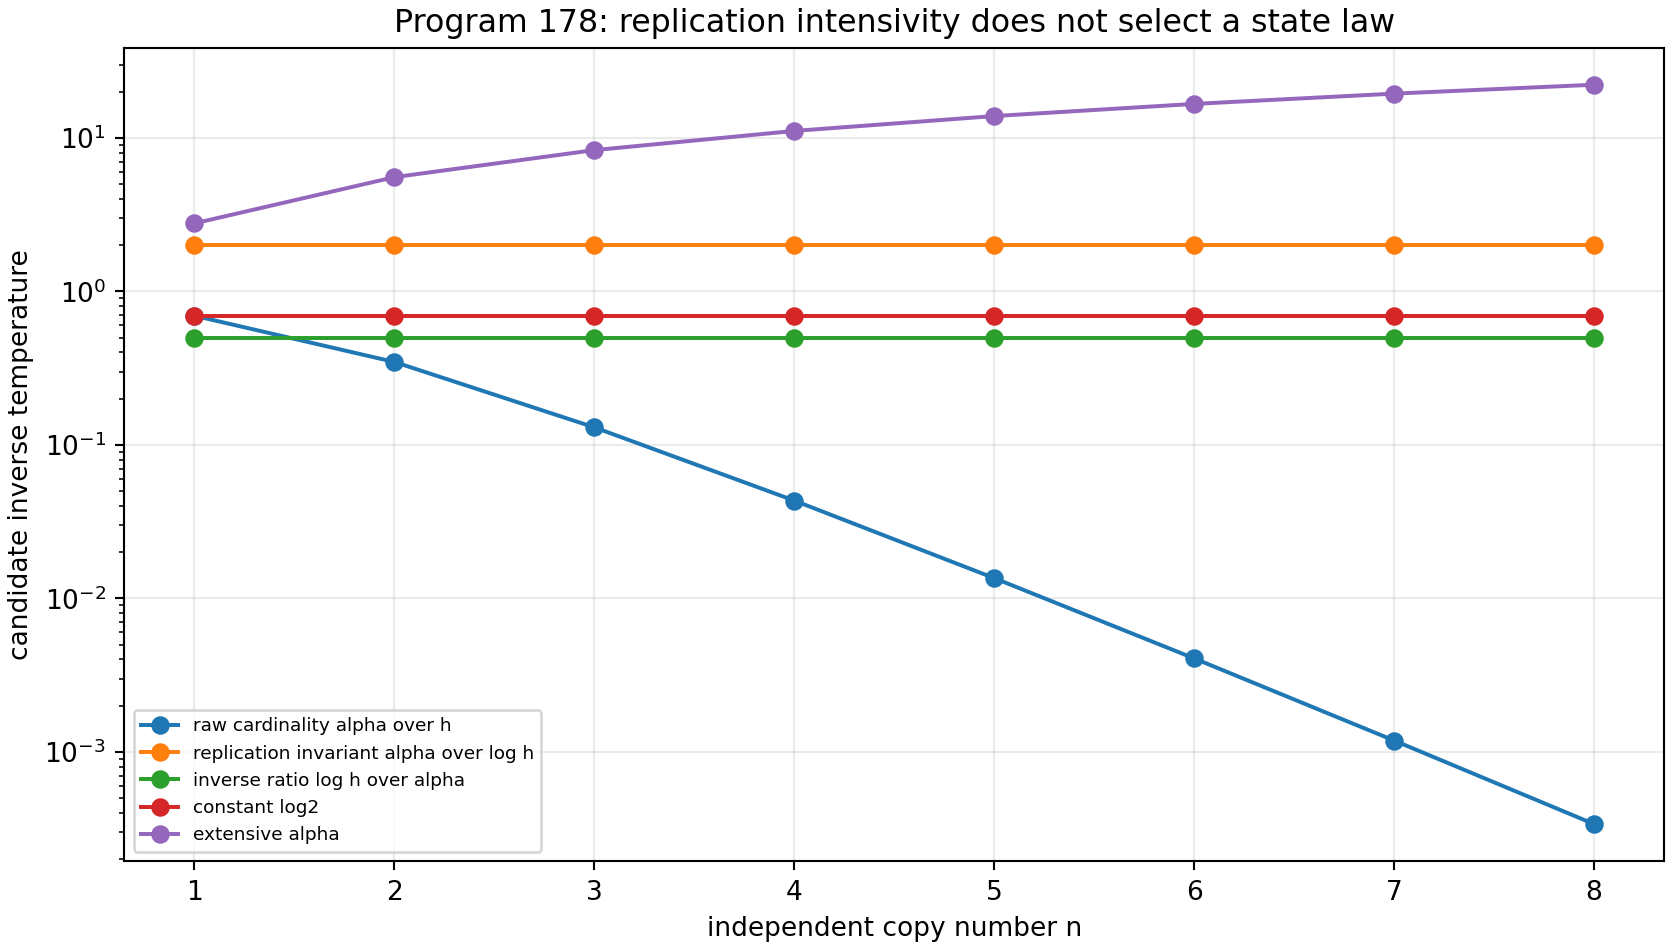
\includegraphics[width=0.94\textwidth]{FIN_Programs_178_190_Composition_Process_Scale_Figures/program178_tensor_intensive_classification.png}
\caption{Replication intensivity leaves multiple state laws; label splitting removes nonconstant ratios without selecting a constant.}
\end{figure}

\section{Verdict}

\textbf{[Proven in the declared continuous scaling class]} Composition does not derive a state temperature. Any successful future state law must introduce a new typed datum, such as a sourced reference state, modular pair or environmental equilibrium condition. Naming \(\log2\) as the surviving constant is target selection, not derivation.

\par\medskip\hrule\medskip

\chapter{Program 179 --- CompressionScaleTorsor}

\section{Scale action}

Consider

\[
D_{\beta,\eta}(d)=\frac1{1+\beta d^\eta},
\qquad\beta>0.
\]

Under \(d'=cd\),

\[
\beta d^\eta
=
\beta c^{-\eta}(d')^\eta.
\]

Thus the positive scaling group acts by

\[
c\cdot\beta=\beta c^{-\eta}.
\]

The action is transitive on \(\mathbb R_{>0}\). Given \(\beta_1,\beta_2>0\), choose

\[
c=(\beta_1/\beta_2)^{1/\eta}.
\]

Then \(c\cdot\beta_1=\beta_2\).

\section{Universal orbit profile}

With

\[
x=\beta^{1/\eta}d,
\]

one obtains

\[
D_{\beta,\eta}(d)=\frac1{1+x^\eta}.
\]

The executable collapses nine values from \(10^{-2}\) to \(10^2\) onto this profile with residual below numerical precision.

\begin{figure}[htbp]
\centering
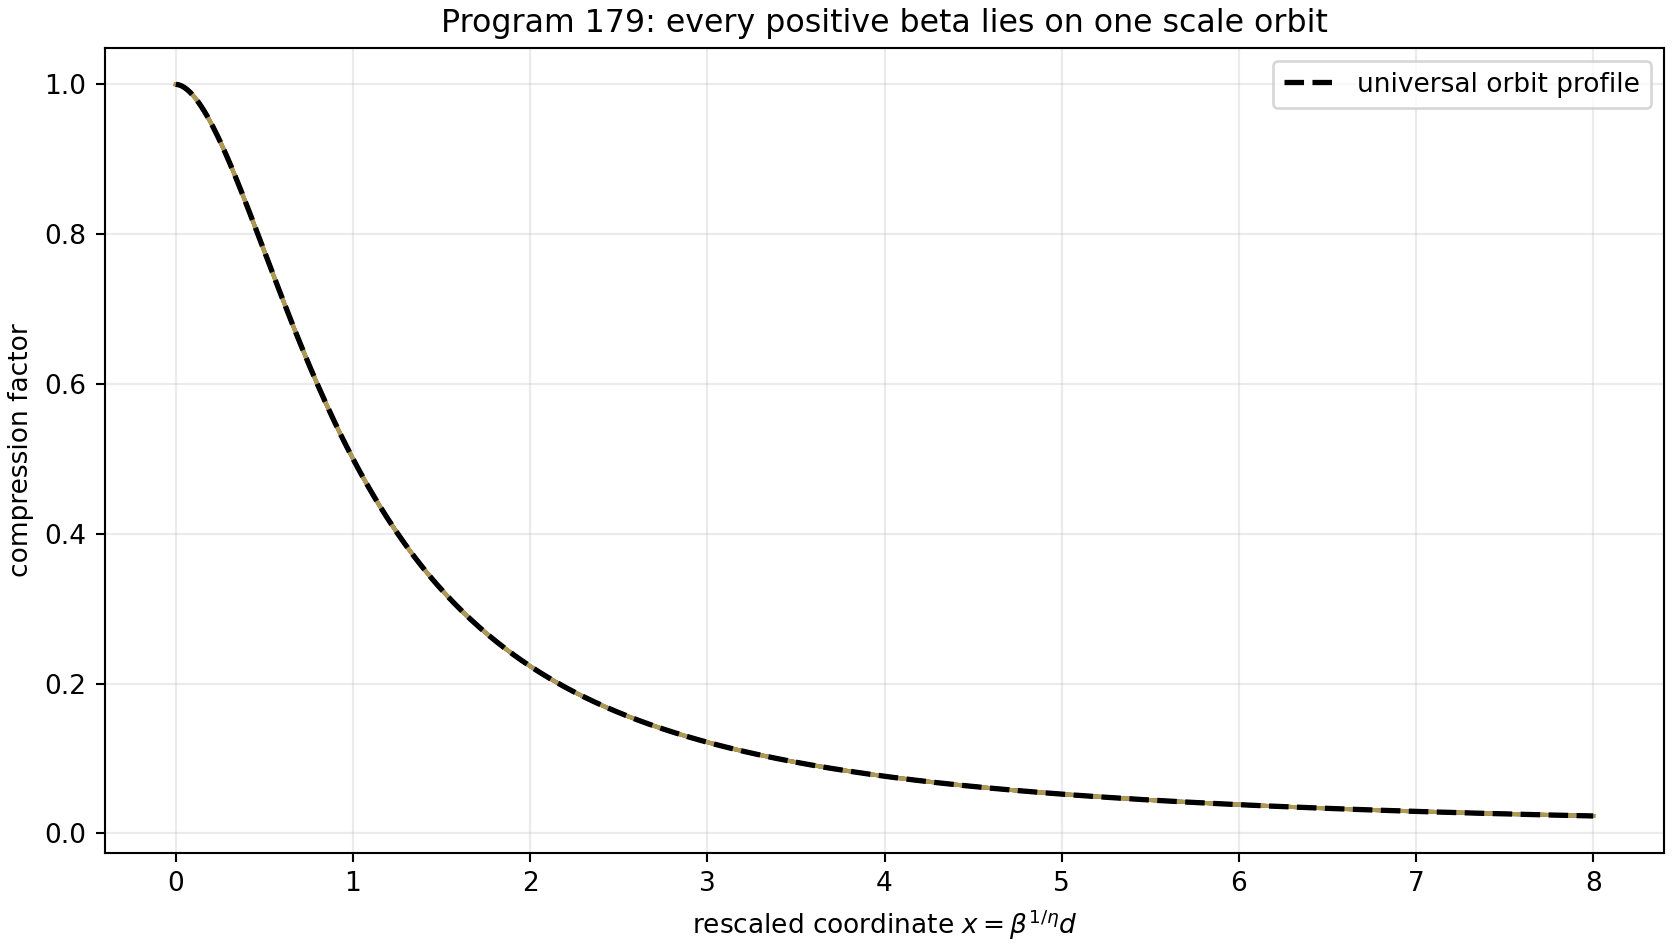
\includegraphics[width=0.94\textwidth]{FIN_Programs_178_190_Composition_Process_Scale_Figures/program179_compression_scale_torsor.png}
\caption{All positive \(\beta\) values collapse to one universal profile after coordinate rescaling.}
\end{figure}

\section{Source audit}

Six routes are tested:

\begin{itemize}
\item 
denominator positivity;

\item 
monoid unitality;

\item 
target tail-ratio inversion;

\item 
the refuted tensor interpretation of \(A_{\rm ME}\);

\item 
the coordinate convention \(\beta=1\);

\item 
an external length calibration.

\end{itemize}

Positivity selects only the positive orbit. Unitality fixes an intercept, not the compression rate. Tail inversion imports the target. \(A_{\rm ME}\) is not tensor-natural. The coordinate convention and external calibration are valid conditional choices but are not strict sources.

\section{Verdict}

\textbf{\statusProven{}} The strict \(\beta\) is a coordinate on CompressionScaleTorsor until a length frame or a genuinely scale-charged source is supplied. Zero accepted target-independent strict sources are exported.

\par\medskip\hrule\medskip

\chapter{Program 180 --- Assembly of the formal fractional certificate}

\section{Components}

The desired certificate must place five pieces in one directed-rounding engine:

\begin{enumerate}
\item 
finite FFT cells;

\item 
the average/\allowbreak{}polylogarithmic term;

\item 
Fourier cancellation modes and their tail;

\item 
denominator replacement;

\item 
resonance fallbacks.

\end{enumerate}

The finite FFT cells already have formal interval status. The cancellation formula is analytic and numerically extremely small:

\[
B_{\rm corr}=4.129713895\times10^{-7}.
\]

The denominator-replacement diagnostic is approximately \(8.48\times10^{-12}\).

\section{Remaining gap}

The previous formal continuous-window enclosure is

\[
R_{\max}=0.6129831478,
\]

whereas the preregistered target is

\[
R_{\max}<0.03.
\]

The new cancellation estimate shows that the oscillatory tail is no longer the dominant conceptual obstacle. What remains is dependency width and the absence of one common ball engine for all components.

\begin{figure}[htbp]
\centering
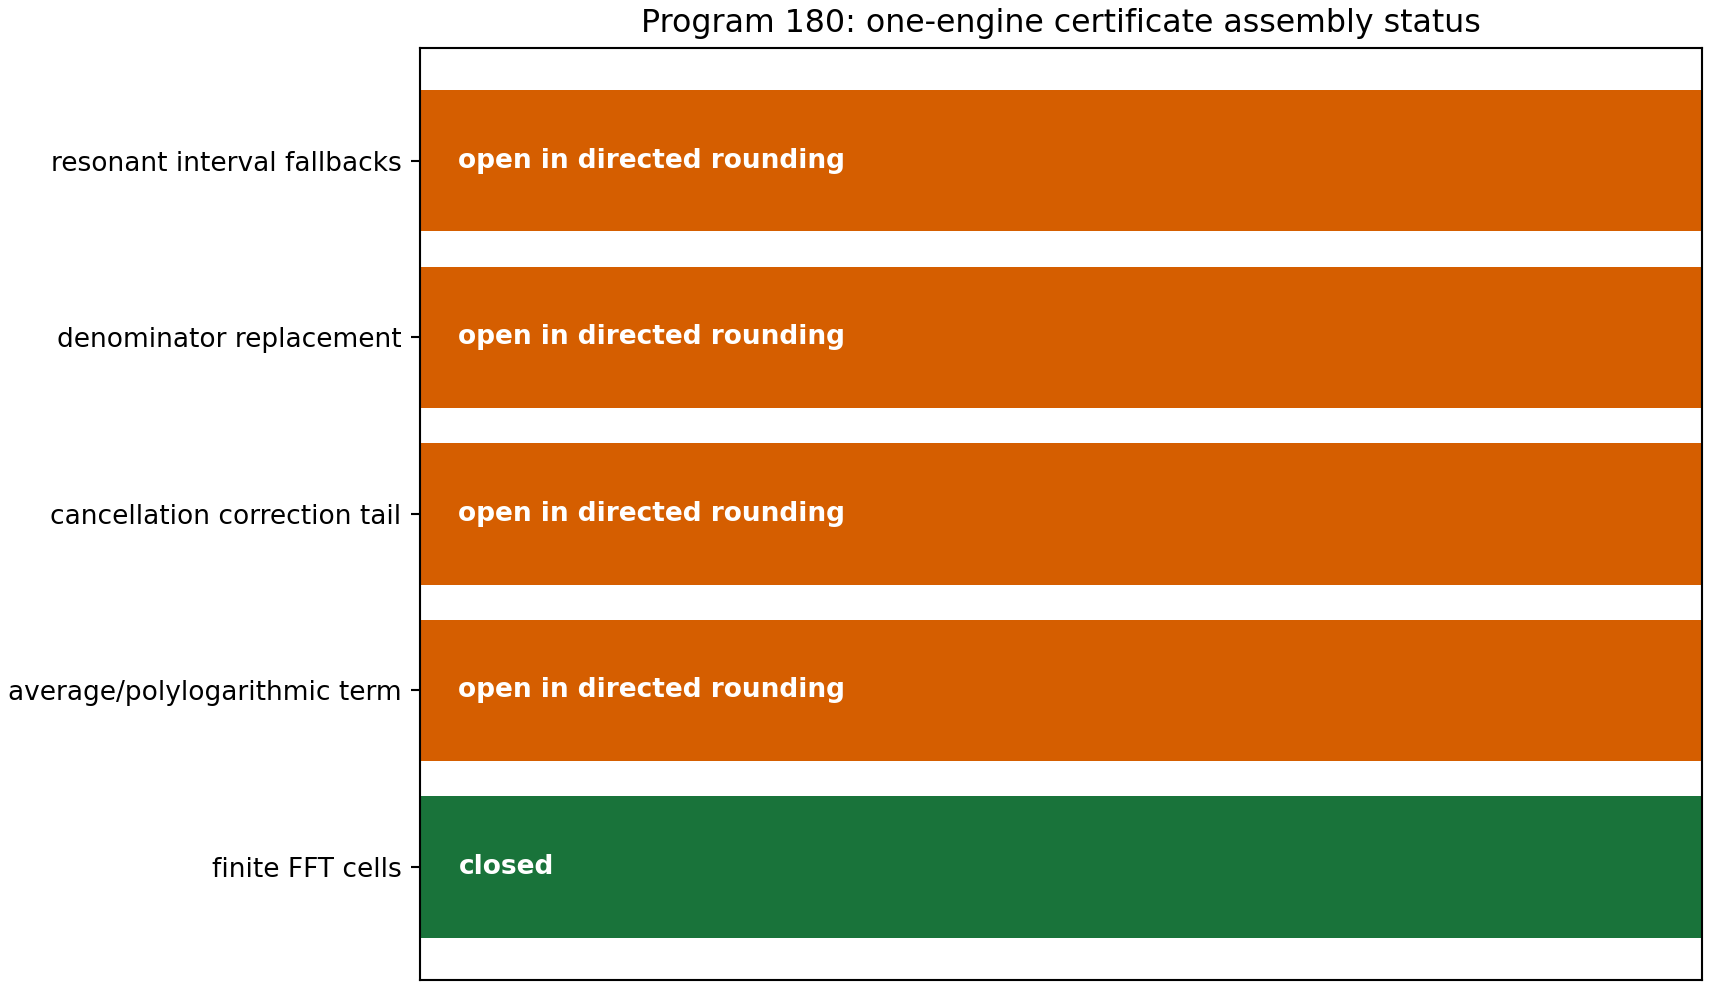
\includegraphics[width=0.94\textwidth]{FIN_Programs_178_190_Composition_Process_Scale_Figures/program180_ball_certificate_ledger.png}
\caption{Only part of the desired fractional certificate currently resides in one directed-rounding chain.}
\end{figure}

\section{Verdict}

\textbf{\statusOpen{}} Arb/\allowbreak{}python-flint is not installed. The program produces an exact obligation ledger and does not falsely convert mixed floating and interval calculations into a formal certificate.

\par\medskip\hrule\medskip

\chapter{Program 181 --- A finite Dirichlet core beyond Boolean AFIS}

\section{Exact graph}

Let \(W\) be the four-cycle transition matrix with weight \(1/2\) on each neighbour and let \(A=I-W\). Then

\[
\operatorname{spec}(A)=\{0,1,1,2\}.
\]

For

\[
f=(1,2,-1,3)^\mathsf T,
\]

exact rational arithmetic gives

\[
f^\mathsf TAf=15
\]

and independently

\[
\frac12\sum_{x,y}W_{xy}(f_x-f_y)^2=15.
\]

Every row of \(A\) sums to zero, hence \(A\mathbf1=0\) exactly.

\section{Dynamics}

Across \(0\le t\le3\), numerical checks give:

\[
\max_t\|U_t^\ast U_t-I\|<2\times10^{-15},
\]

and heat-kernel row-sum residual below \(10^{-15}\), with no significant negative entry.

\begin{figure}[htbp]
\centering
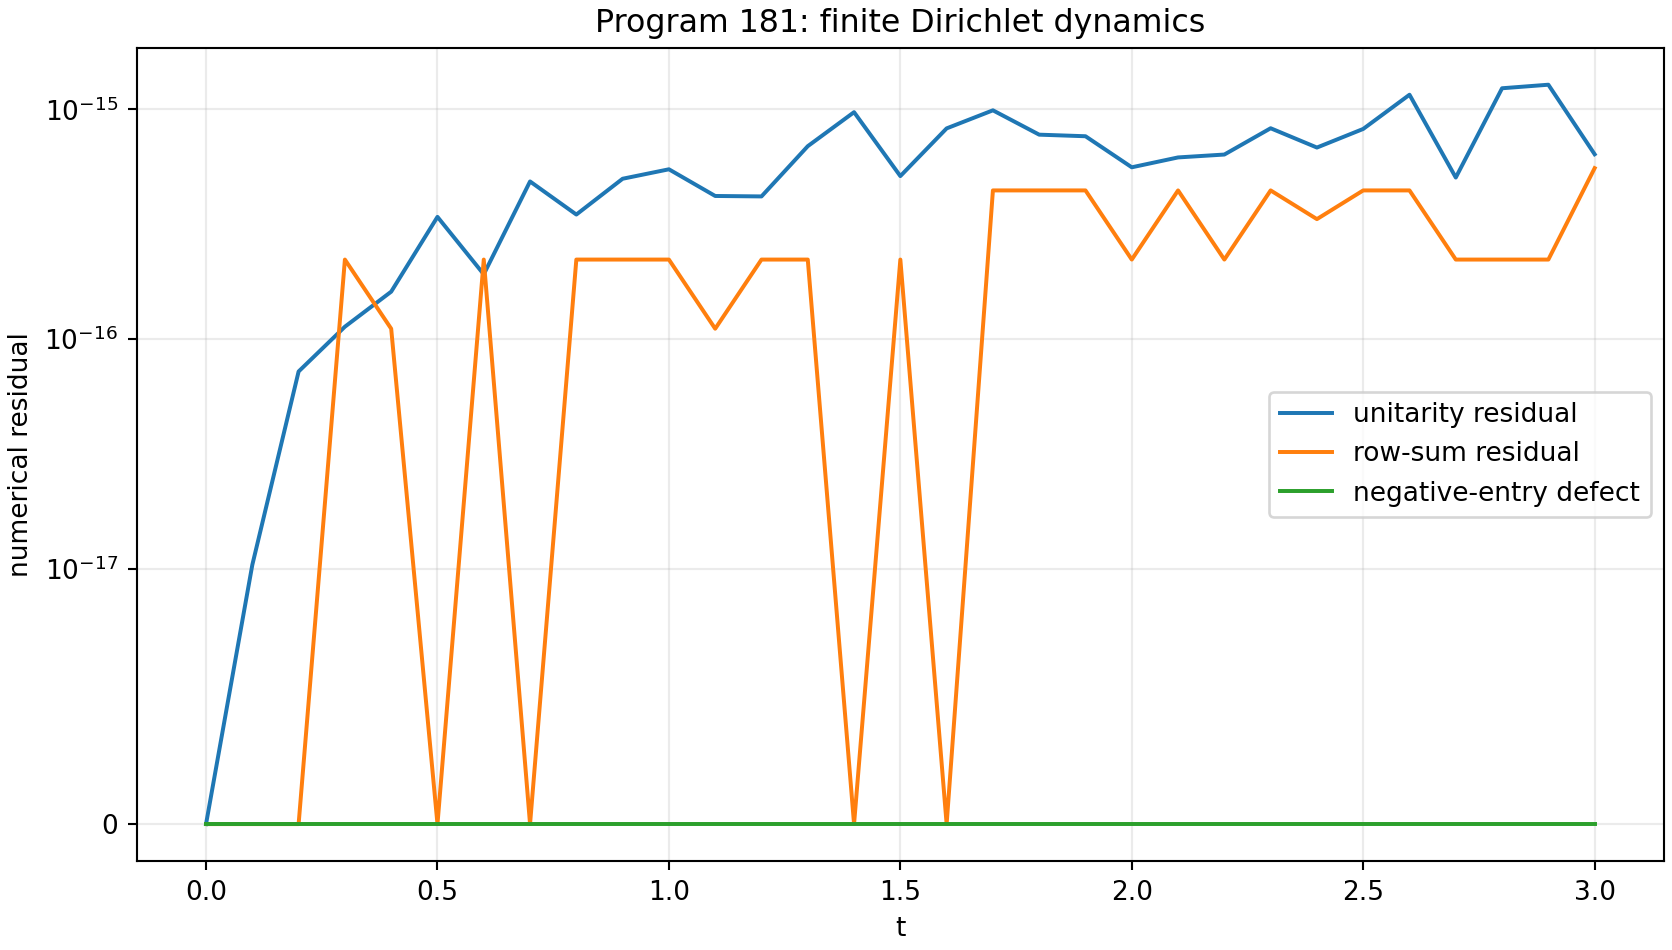
\includegraphics[width=0.94\textwidth]{FIN_Programs_178_190_Composition_Process_Scale_Figures/program181_dirichlet_core.png}
\caption{Unitarity, heat row sums and heat positivity for the exact four-cycle Dirichlet generator.}
\end{figure}

\section{Formal artifact}

The Lean source defines the four-cycle Dirichlet energy, proves the constant-vector statement and records the concrete integer energy calculation. Because the Lean toolchain is not locally installed after the documented download failures, the file is not reported as machine-compiled.

\section{Verdict}

\textbf{\statusProven{}} The exact finite mathematics is independent of the earlier Boolean capability model. \textbf{\statusOpen{}} A proof-assistant development of general weighted matrices, functional calculus and positivity-preserving semigroups still requires an installed mathematical library.

\par\medskip\hrule\medskip

\chapter{Program 182 --- Complete reflection-covariant qubit conversion}

\section{Choi normal form}

Reflection is conjugation by \(\sigma_z\). A covariant qubit channel has a Choi matrix commuting with \(\sigma_z\otimes\sigma_z\). In input--output basis it has the X form

\[
J=
\begin{pmatrix}
a&0&0&w\\
0&1-a&\zeta&0\\
0&\bar\zeta&c&0\\
\bar w&0&0&1-c
\end{pmatrix}.
\]

Trace preservation is already encoded. Complete positivity is equivalent to

\[
0\le a,c\le1,
\]

\[
|w|^2\le a(1-c),\qquad
|\zeta|^2\le(1-a)c.
\]

\section{Conversion criterion}

Use free rotations about the \(z\) axis to align transverse phases. Write the source and target Bloch data as \((r,z)\) and \((r',z')\), with

\[
p=\frac{1+z}{2},\qquad p'=\frac{1+z'}2.
\]

A covariant conversion exists if and only if some \(a,c\in[0,1]\) satisfy

\[
p'=pa+(1-p)c
\]

and

\[
r'\le
r\left[
\sqrt{a(1-c)}+\sqrt{(1-a)c}
\right].
\]

Necessity follows from the two Choi minors. Sufficiency follows by choosing the phases of \(w\) and \(\zeta\) to align and saturating only as much coherence as needed.

\section{Counterexample completed}

For source \((r,z)=(0.6,0)\) and target \((0.6,0.8)\), the population constraint requires \(a+c=1.8\). The maximal bracket is \(0.6\), hence

\[
r'_{\max}=0.6\times0.6=0.36.
\]

The target value \(0.6\) is unreachable even though the old monotone has the same value on source and target. In the declared target grid, 1,366 valid cells pass the scalar \(M\) test but fail the complete criterion.

\begin{figure}[htbp]
\centering
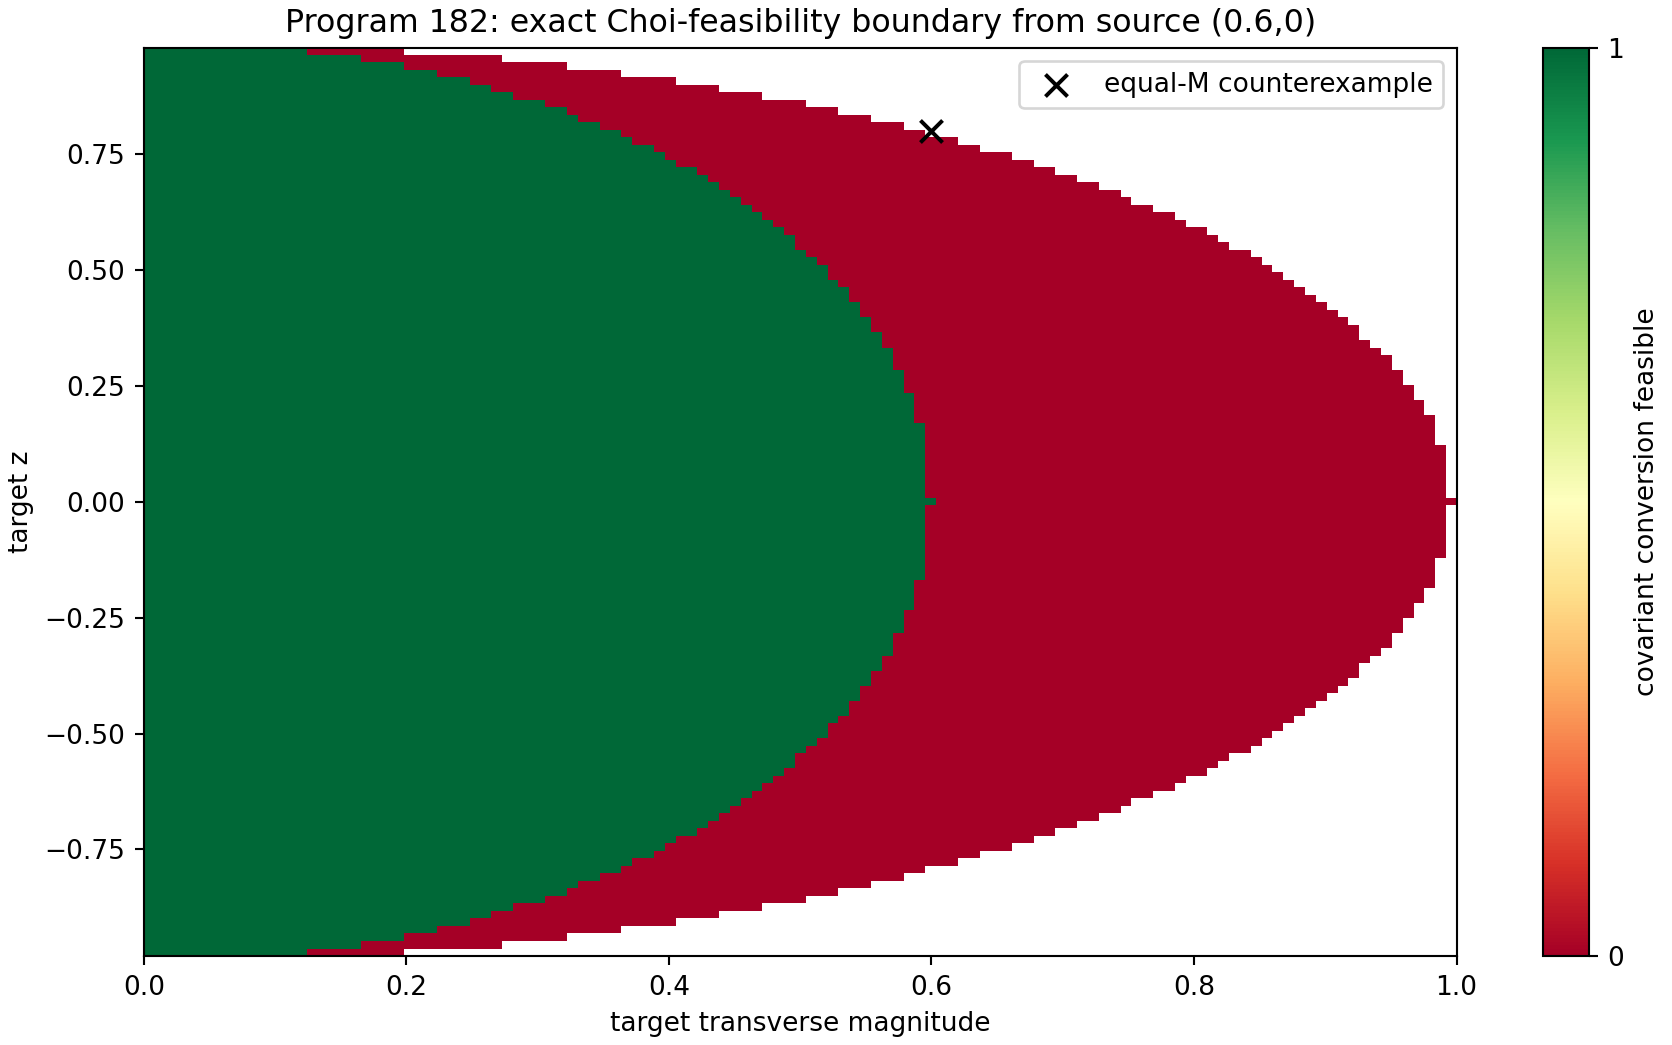
\includegraphics[width=0.94\textwidth]{FIN_Programs_178_190_Composition_Process_Scale_Figures/program182_reflection_convertibility.png}
\caption{Complete Choi-feasibility region from the source Bloch state with transverse coordinate 0.6.}
\end{figure}

\section{Verdict}

\textbf{\statusProven{}} The new LMI is complete for deterministic single-qubit reflection-covariant conversion. It classifies a supplied resource; it does not create a signed preparation or select a polarity.

\par\medskip\hrule\medskip

\chapter{Program 183 --- Dependence-robust DKW for repeated blocks}

\section{Exact dependence class}

Let \(Y_1,\ldots,Y_m\) be iid, and form a record by repeating each \(Y_j\) exactly \(b\) times in one contiguous block. Then

\[
F_n(x)
=
\frac1{mb}\sum_{j=1}^m b\,\mathbf1\{Y_j\le x\}
=
\frac1m\sum_{j=1}^m\mathbf1\{Y_j\le x\}.
\]

The empirical CDF is exactly the \(m\)-sample CDF. Therefore

\[
\Pr(\|F_n-F\|_\infty>\epsilon)
\le2e^{-2m\epsilon^2}.
\]

Using nominal \(n=mb\) is mathematically wrong.

\section{Executed challenge}

For \(m=40\), \(b=100\), \(n=4000\) and two time cells:

\[
\epsilon_n=0.0234041,\qquad
\epsilon_m=0.234041.
\]

Across 360 stable-law repetitions:

\[
\text{nominal coverage}=0.625,
\]

\[
\text{block-valid coverage}=1.000.
\]

The mean interval width rises from \(0.516\) to \(10.579\).

\begin{figure}[htbp]
\centering
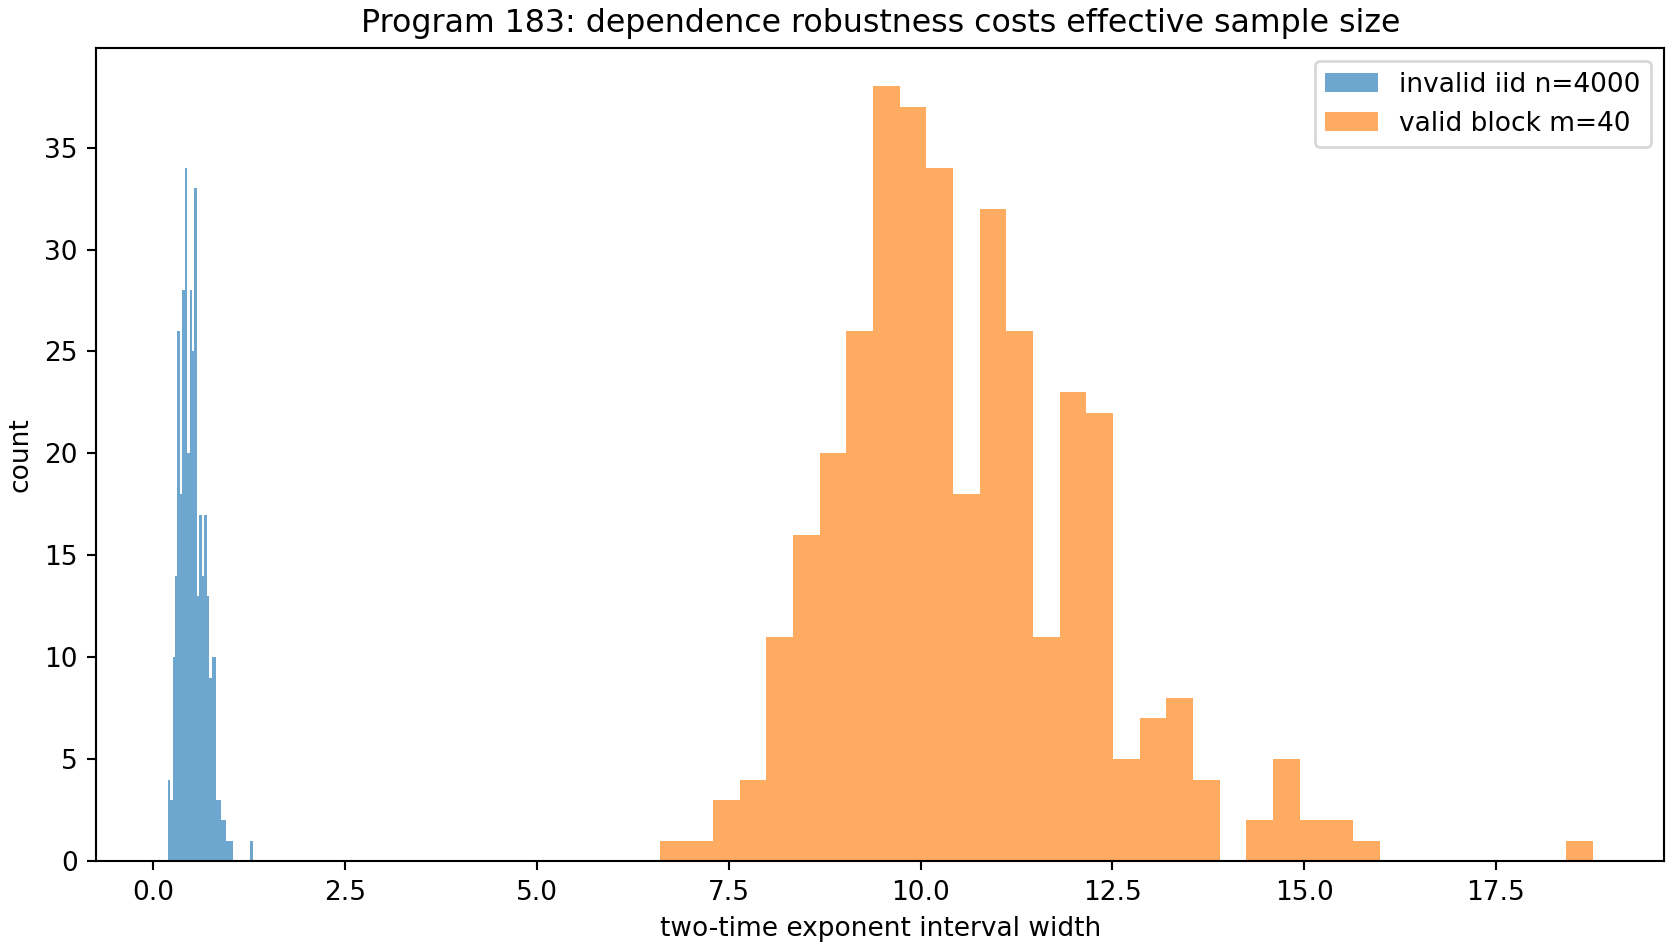
\includegraphics[width=0.94\textwidth]{FIN_Programs_178_190_Composition_Process_Scale_Figures/program183_block_DKW.png}
\caption{Correct dependence coverage requires the number of independent blocks and produces much wider intervals.}
\end{figure}

\section{Interpretation}

\textbf{\statusProven{}} Correct coverage is recovered for the declared block model. The price is an almost uninformative interval. Dependence cannot be repaired by changing a label on \(n\); the acquisition protocol must certify the number of independent units.

\par\medskip\hrule\medskip

\chapter{Program 184 --- Nonlinear multi-control calibration}

\section{Model}

Let \(x=\log t\) and take

\[
\log Q_j(x)
=
a_j+T_jx+g_1x+g_2x^2.
\]

The target exponent \(T\) is unknown. Two controls have independently known exponents \(T_{C1}=0.5\) and \(T_{C2}=1.0\). At \(x\in\{-1,0,1\}\), the parameter vector is

\[
(a_T,a_{C1},a_{C2},T,g_1,g_2).
\]

The nine-cell design has rank six.

\section{Role of the second control}

Inside the exact shared-gain model, one control at three times already gives rank five for its reduced parameter set. The second control is not falsely called algebraically necessary. Its role is scientific falsification: after subtracting the known exponents, the two control slopes must agree.

\section{Simulation}

With \(T=1.25\), \(g_1=0.7\), \(g_2=0.35\), twelve observations per cell and 1,500 repetitions:

\[
\overline T_{\rm naive}=1.949629,
\]

\[
\overline T_{\rm calibrated}=1.249501,
\]

\[
\operatorname{sd}(\widehat T)=0.029930.
\]

Adding a control-specific gain defect \(0.25\) is detected by the cross-control contrast in all declared trials.

\begin{figure}[htbp]
\centering
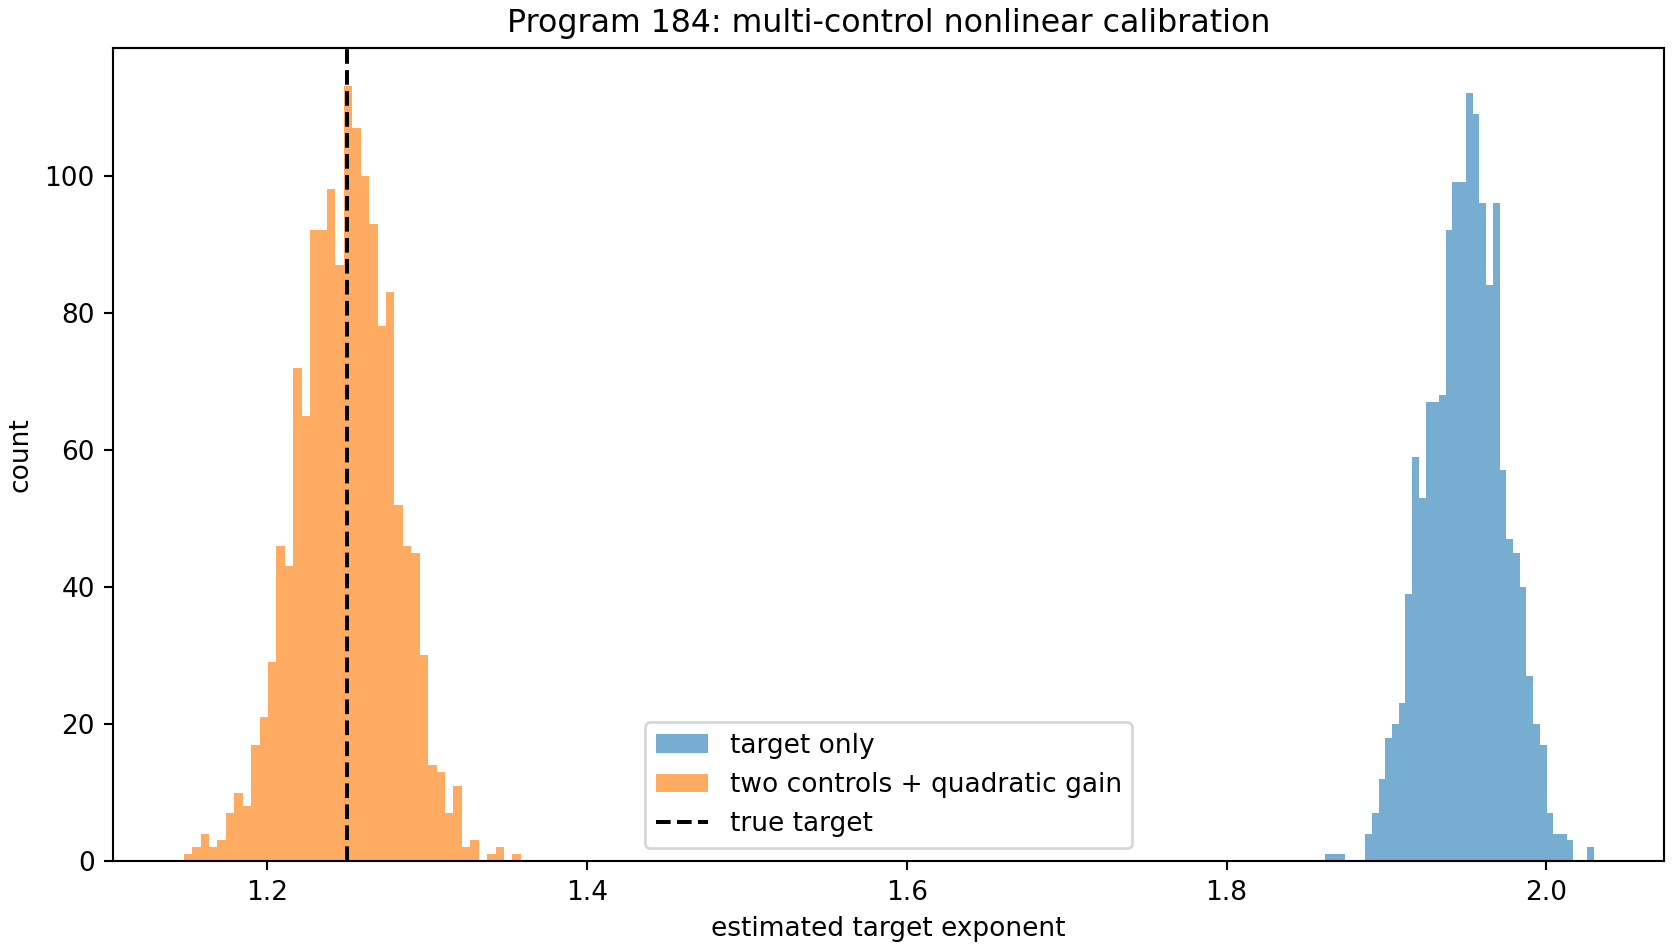
\includegraphics[width=0.94\textwidth]{FIN_Programs_178_190_Composition_Process_Scale_Figures/program184_multi_control.png}
\caption{Known controls remove shared nonlinear detector gain from the target exponent.}
\end{figure}

\section{Verdict}

\textbf{[Proven rank; strong synthetic evidence]} The constructed MultiControlCalibrationFrame separates quadratic apparatus response and makes one important nuisance assumption testable. It remains conditional on the chosen response family.

\par\medskip\hrule\medskip

\chapter{Program 185 --- Open-set challenge and a feature impossibility theorem}

\section{Frozen challenge}

The classifier, feature scales, class centroids and abstention thresholds from Program 174 are left unchanged. Four unseen generators are declared before execution:

\begin{itemize}
\item 
ordered/\allowbreak{}correlated Gaussian records;

\item 
tempered stable \(\alpha=0.8\);

\item 
Gaussian--Cauchy mixtures;

\item 
nonshared random detector gain.

\end{itemize}

\section{Exact order-blindness}

Every frozen feature is a function of one-time empirical quantiles or boundary atom counts. Hence it depends only on the multiset of values, not their ordering. For every permutation \(\pi\),

\[
\Phi(x_1,\ldots,x_n)
=
\Phi(x_{\pi(1)},\ldots,x_{\pi(n)}).
\]

Sorting the records creates strong temporal organization while preserving the features exactly. The observed maximum feature difference is zero.

\section{Results}

The ordered Gaussian class is rejected only \(6.11\%\) of the time and falsely accepted \(93.89\%\) of the time, almost always as local Gaussian. The other three declared unknowns are rejected at rates between \(98.33\%\) and \(100\%\).

\begin{figure}[htbp]
\centering
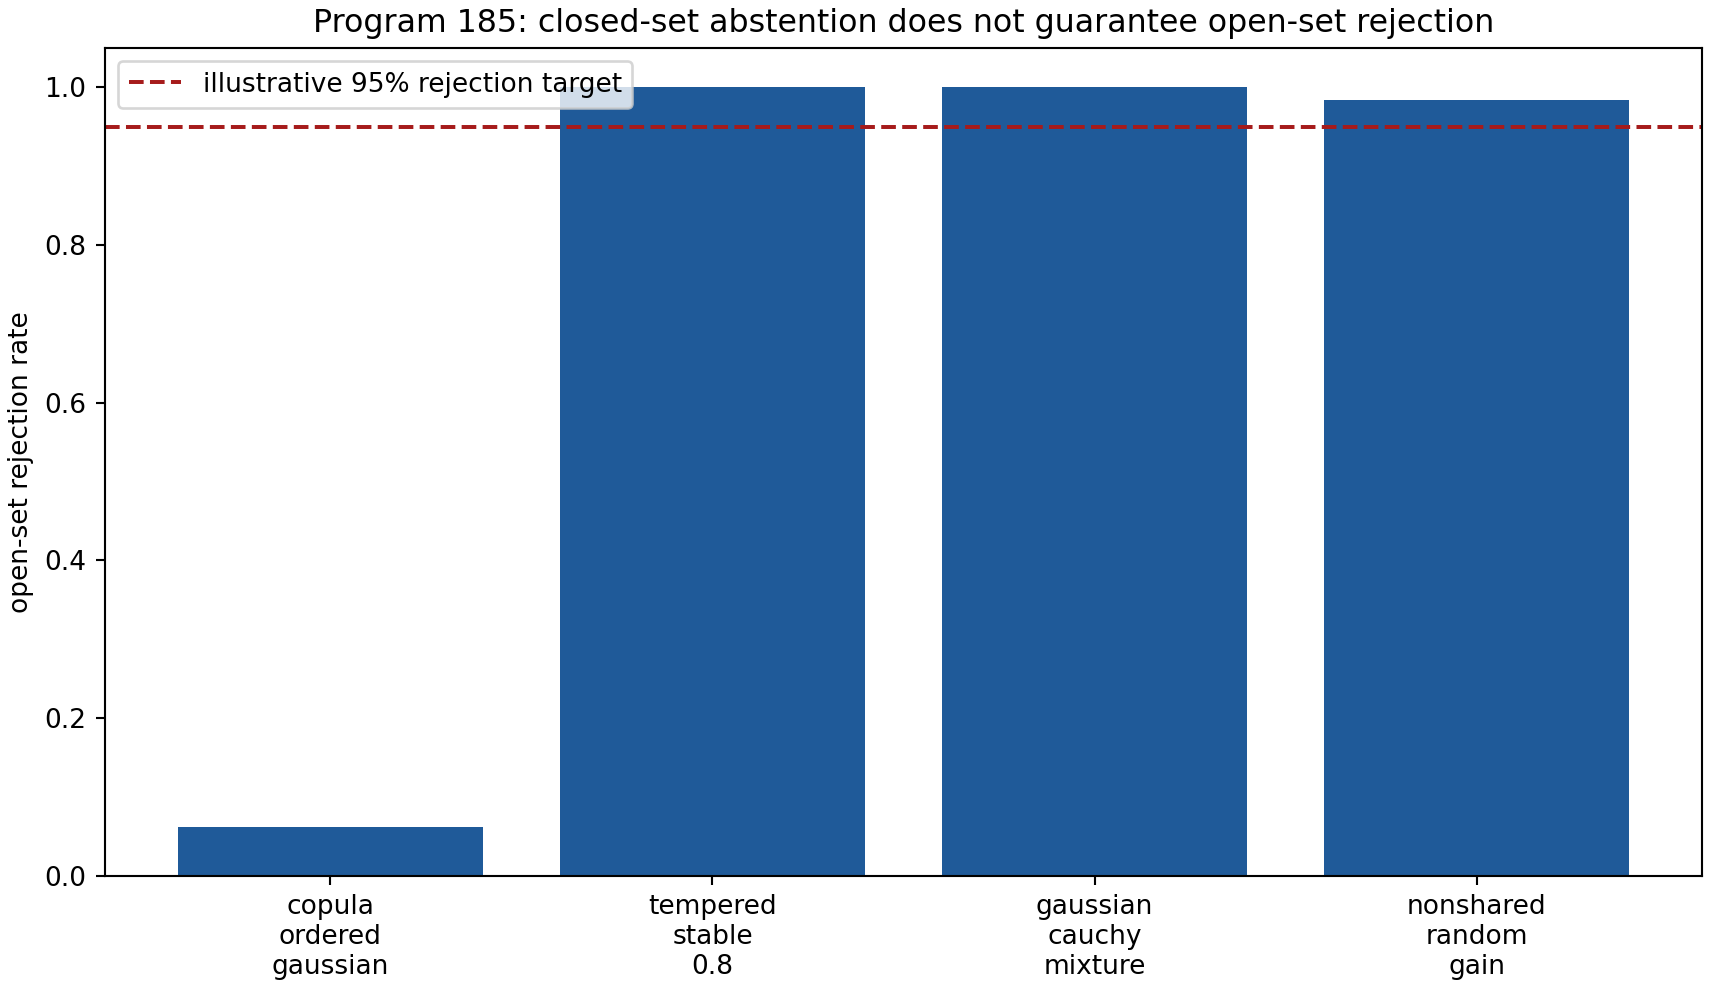
\includegraphics[width=0.94\textwidth]{FIN_Programs_178_190_Composition_Process_Scale_Figures/program185_open_set.png}
\caption{Closed-set distance thresholds reject several unseen laws but cannot reject a feature-invariant ordering challenge.}
\end{figure}

\section{Verdict}

\textbf{\statusProven{}} No classifier based solely on the frozen marginal features can identify temporal memory. Good rejection of some unseen marginal laws does not repair this exact invariance. The next protocol must add ordering-sensitive features or explicit interventions.

\par\medskip\hrule\medskip

\chapter{Program 186 --- TwoStepProcessInstrument for double slit}

\section{Memoryful phase process}

Let a quasistatic Gaussian phase \(\xi\) have variance \(\sigma^2\), constant across two intervals. Coherence after time \(t\) is

\[
\Gamma(t)=\mathbb E(e^{i\xi t})
=e^{-\sigma^2t^2/2}.
\]

For \(\sigma=0.8\) and \(t_1=t_2=1\):

\[
\Gamma_1=\Gamma_2=0.726149,
\]

\[
\Gamma_{12}^{\rm static}=e^{-1.28}=0.278037.
\]

A Markov process matched at one step gives

\[
\Gamma_{12}^{\rm Markov}
=\Gamma_1\Gamma_2
=0.527292.
\]

The nonfactorization witness is

\[
\mathcal M
=\Gamma_{12}^{\rm static}
-\Gamma_1\Gamma_2
=-0.249255.
\]

\section{Echo intervention}

Reversing the path phase sign between intervals cancels a static phase:

\[
\Gamma_{\rm echo}^{\rm static}=1.
\]

Independent Markov increments are not refocused:

\[
\Gamma_{\rm echo}^{\rm Markov}=0.527292.
\]

Detector blur gives a separate visibility transfer \(0.84\), while a localized path preparation supplies a population-survival contrast for classical path diffusion.

\begin{figure}[htbp]
\centering
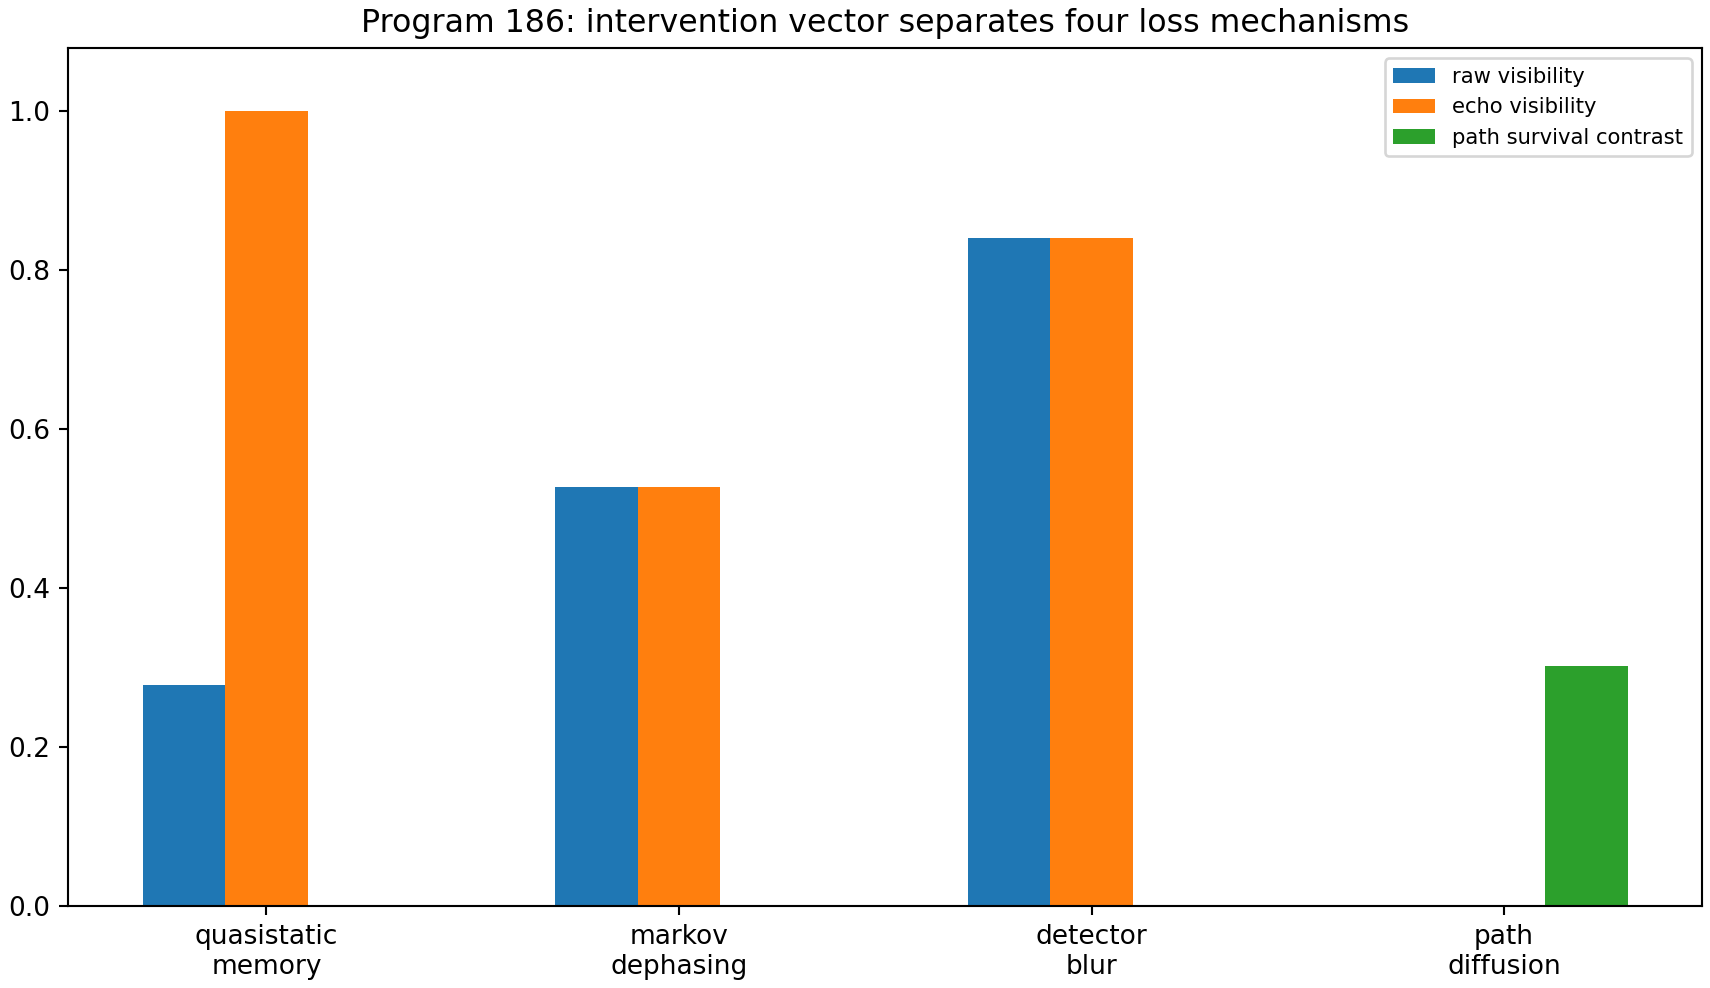
\includegraphics[width=0.94\textwidth]{FIN_Programs_178_190_Composition_Process_Scale_Figures/program186_process_tensor.png}
\caption{A three-component intervention vector separates four declared visibility-loss mechanisms.}
\end{figure}

\section{Constructed object}

TwoStepProcessInstrument contains:

\begin{itemize}
\item 
path preparation;

\item 
a two-step random-unitary process;

\item 
optional echo intervention;

\item 
path-population control;

\item 
phase POVM;

\item 
detector calibration;

\item 
persistent record.

\end{itemize}

\section{Verdict}

\textbf{[Conditional; proven finite formulas]} The intervention vector separates four declared mechanisms. It does not follow from the kernel alone and is not device-independent or externally validated.

\par\medskip\hrule\medskip

\chapter{Program 187 --- Environment nonuniqueness}

\section{Explicit dilation family}

Keep the path generator \(A\) fixed. Let an environment qubit start in \(|+\rangle\) and use

\[
V_g
=
|0\rangle\langle0|\otimes I
+
|1\rangle\langle1|\otimes e^{-ig\sigma_z}.
\]

Tracing out the environment yields

\[
\rho_{01}\longmapsto
\langle+|e^{-ig\sigma_z}|+\rangle\rho_{01}
=
\cos(g)\rho_{01}.
\]

For every \(0\le g\le\pi/2\) this is a valid dephasing channel. Its normalized Choi eigenvalues are

\[
\left(
\frac{1+\cos g}{2},
\frac{1-\cos g}{2},
0,0
\right).
\]

\begin{figure}[htbp]
\centering
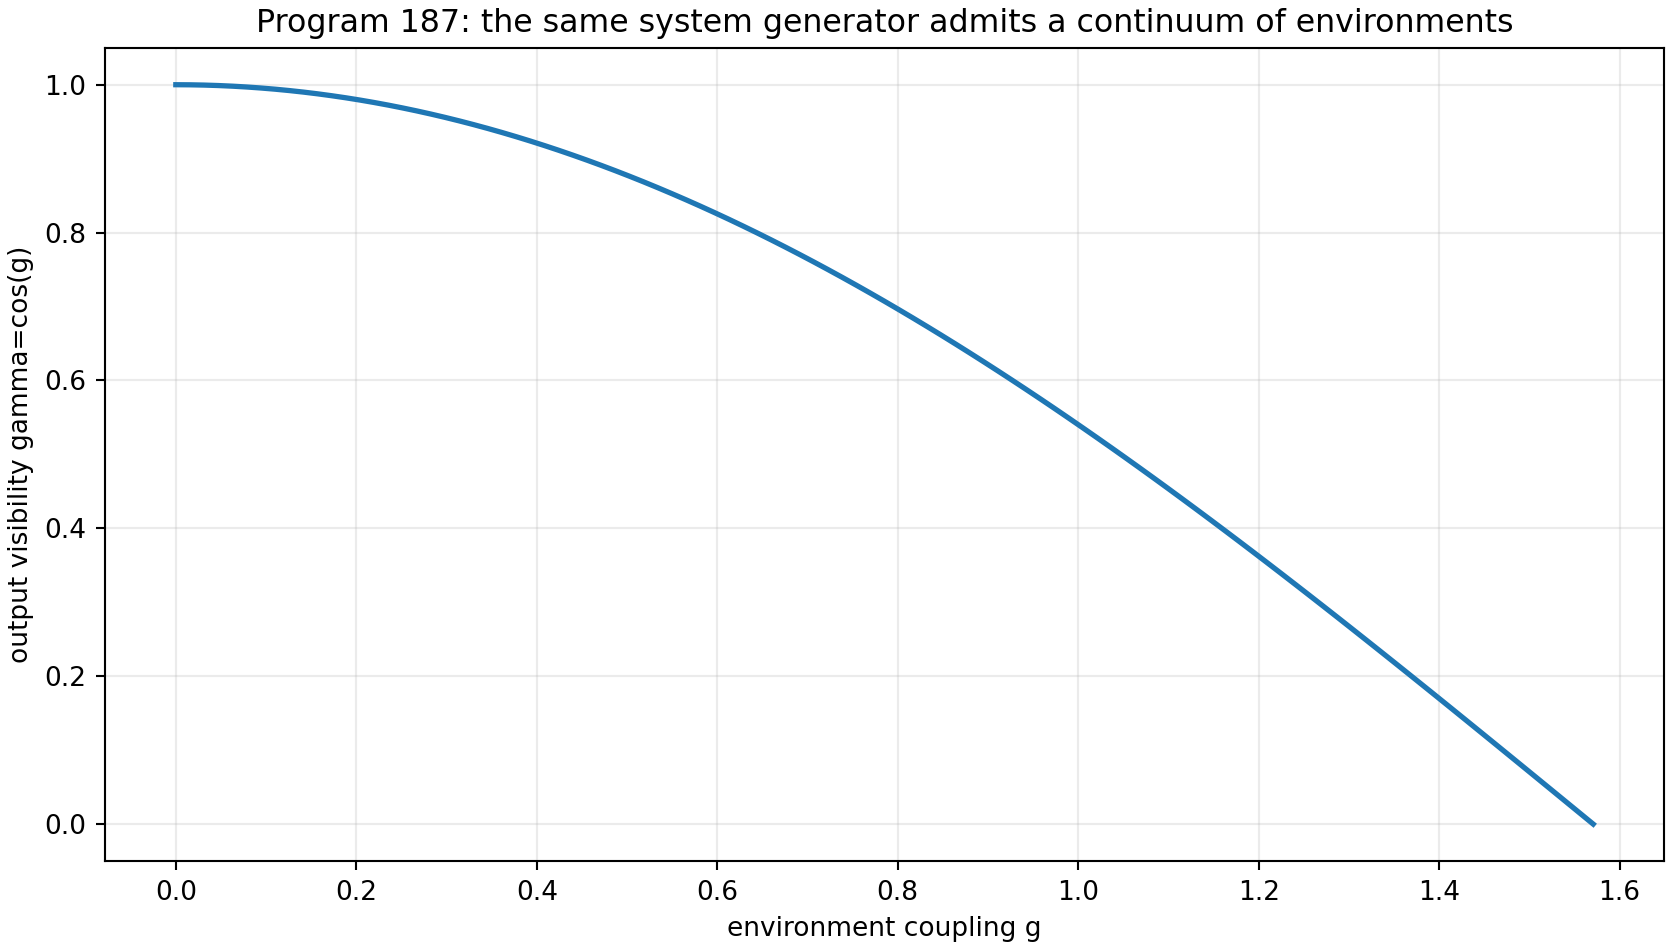
\includegraphics[width=0.94\textwidth]{FIN_Programs_178_190_Composition_Process_Scale_Figures/program187_environment_nonuniqueness.png}
\caption{One fixed system generator admits a continuum of environment couplings and dephasing visibilities.}
\end{figure}

\section{No-go theorem}

The system operator \(A\) contains no value of \(g\). Holding \(A\) fixed while varying \(g\) changes visibility continuously from one to zero. Therefore a unique environment, channel or record cannot be a function of \(A\) alone.

\section{Minimal replacement}

Microscopic dilations contain operationally redundant information. The minimal observer-facing object is

\[
\text{EnvironmentProcessClass}
=
\frac{\{\text{dilations}\}}
{\text{same reduced process tensor}}.
\]

\textbf{\statusProven{}} This quotient is a more economical missing object than a preferred microscopic environment, but the reduced process still has to be specified or sourced.

\par\medskip\hrule\medskip

\chapter{Program 188 --- Cohomology and transcendence of the phase correction}

\section{Character classes}

For trivial coefficients,

\[
H^1(\mathbb Z,U(1))
=
\operatorname{Hom}(\mathbb Z,U(1))
\cong U(1).
\]

A character is fixed by the image of the generator.

The legacy value

\[
\lambda_\ell=e^{i\pi/4}
\]

is an algebraic eighth root of unity. The strict value

\[
\lambda_s=e^{i743/4000}
\]

is transcendental because \(i743/4000\) is a nonzero algebraic number and Lindemann--Weierstrass makes its exponential transcendental.

\section{Algebraic source obstruction}

The correction generator is

\[
\lambda_C
=
\frac{\lambda_s}{\lambda_\ell}.
\]

If \(\lambda_C\) were algebraic, then \(\lambda_s=\lambda_C\lambda_\ell\) would be algebraic, contradiction. Therefore \(\lambda_C\) is transcendental.

Finite algebraic operations on the legacy cyclotomic field remain algebraic. They cannot produce \(\lambda_s\) or \(\lambda_C\).

The constant offset

\[
\Delta\phi=\frac{13}{80}-\frac{\pi}{6}
\]

is an affine phase-origin correction, not part of a normalized group character.

\begin{figure}[htbp]
\centering
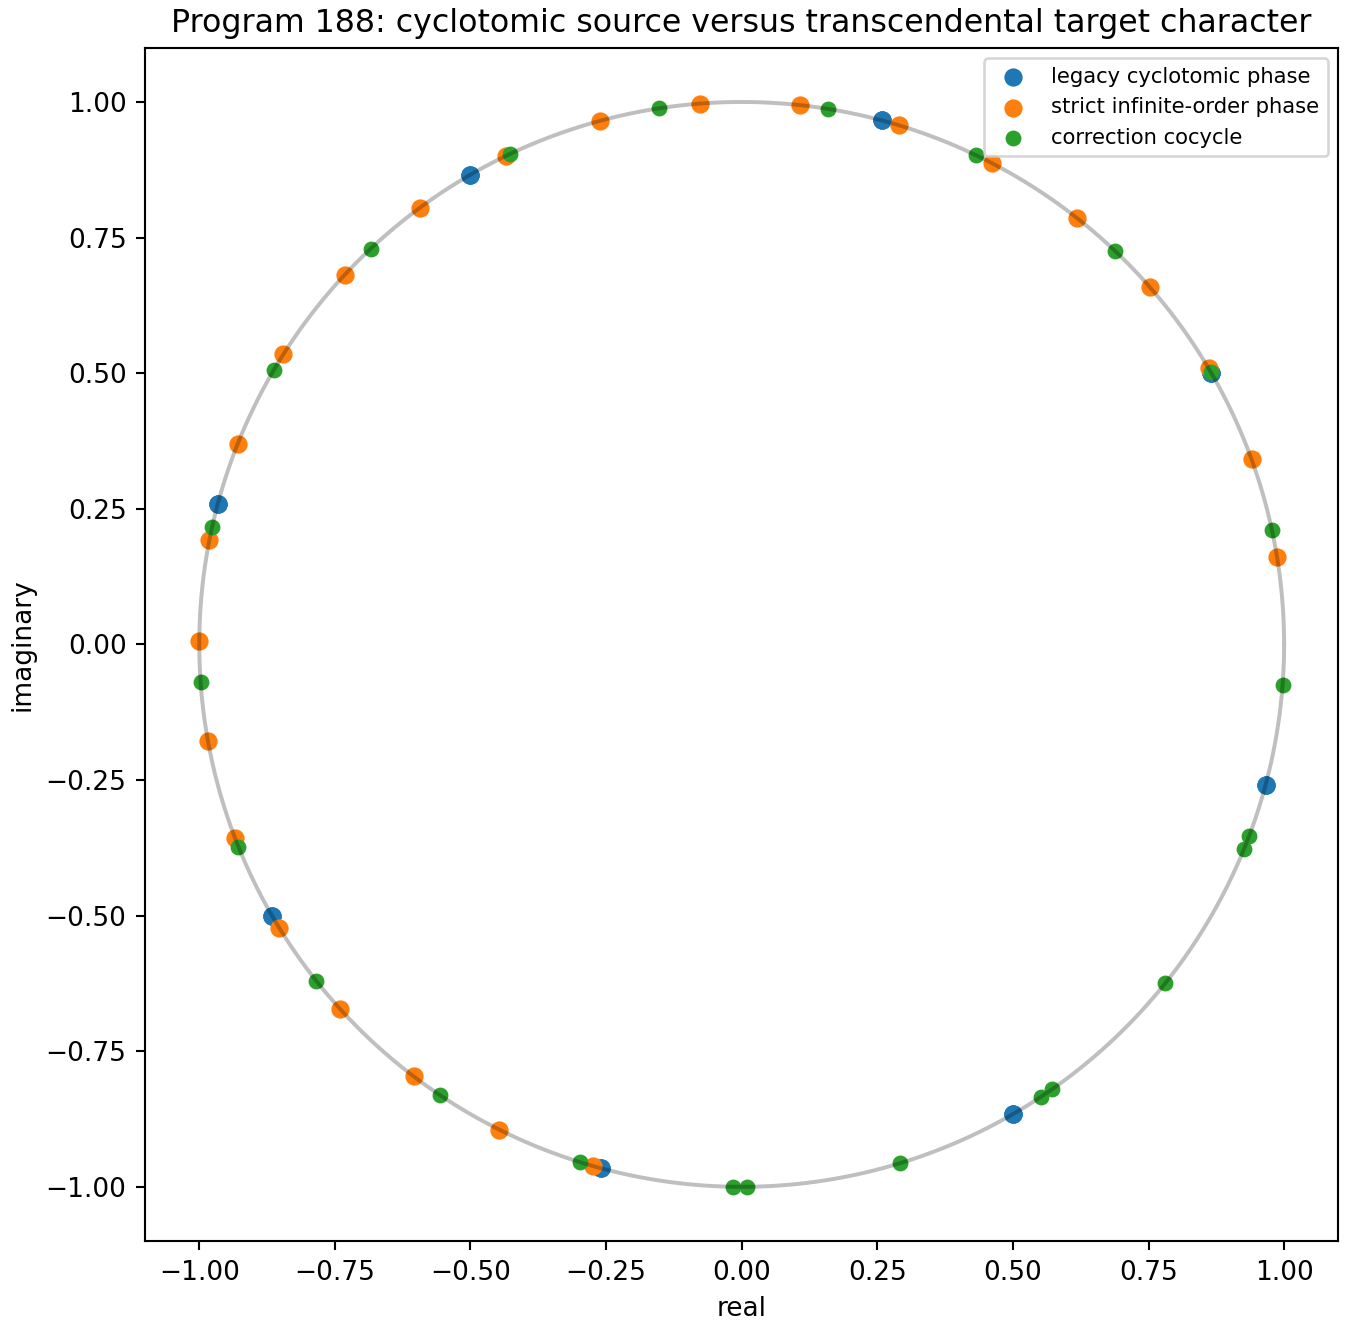
\includegraphics[width=0.94\textwidth]{FIN_Programs_178_190_Composition_Process_Scale_Figures/program188_phase_cohomology.png}
\caption{Legacy cyclotomic, strict infinite-order and correction phase values on the unit circle.}
\end{figure}

\section{Verdict}

\textbf{\statusProven{}} An algebraic legacy-only completion is impossible. A future bridge needs genuinely new analytic data and a sourced phase origin. The target quotient supplies the answer but not its cause.

\par\medskip\hrule\medskip

\chapter{Program 189 --- Intrinsic scale-orbit obstruction}

\section{Symmetry}

For \(c>0\) define

\[
A_c=cA,\qquad t_c=t/c,\qquad z_c=cz.
\]

Then

\[
e^{-it_cA_c}=e^{-itA},
\]

\[
e^{-t_cA_c}=e^{-tA},
\]

and

\[
c(A_c+z_cI)^{-1}=(A+zI)^{-1}.
\]

Thus every normalized prediction is constant on a free \(\mathbb R_{>0}\) orbit.

\section{Executed orbit}

Across \(10^{-3}\le c\le10^3\):

\begin{itemize}
\item 
unitary residual is below \(4\times10^{-16}\);

\item 
heat residual is below \(3\times10^{-16}\);

\item 
resolvent covariance residual is below \(3\times10^{-15}\);

\item 
the normalized gap is constant to approximately \(5\times10^{-16}\);

\item 
the raw gap changes by a factor \(10^6\).

\end{itemize}

\begin{figure}[htbp]
\centering
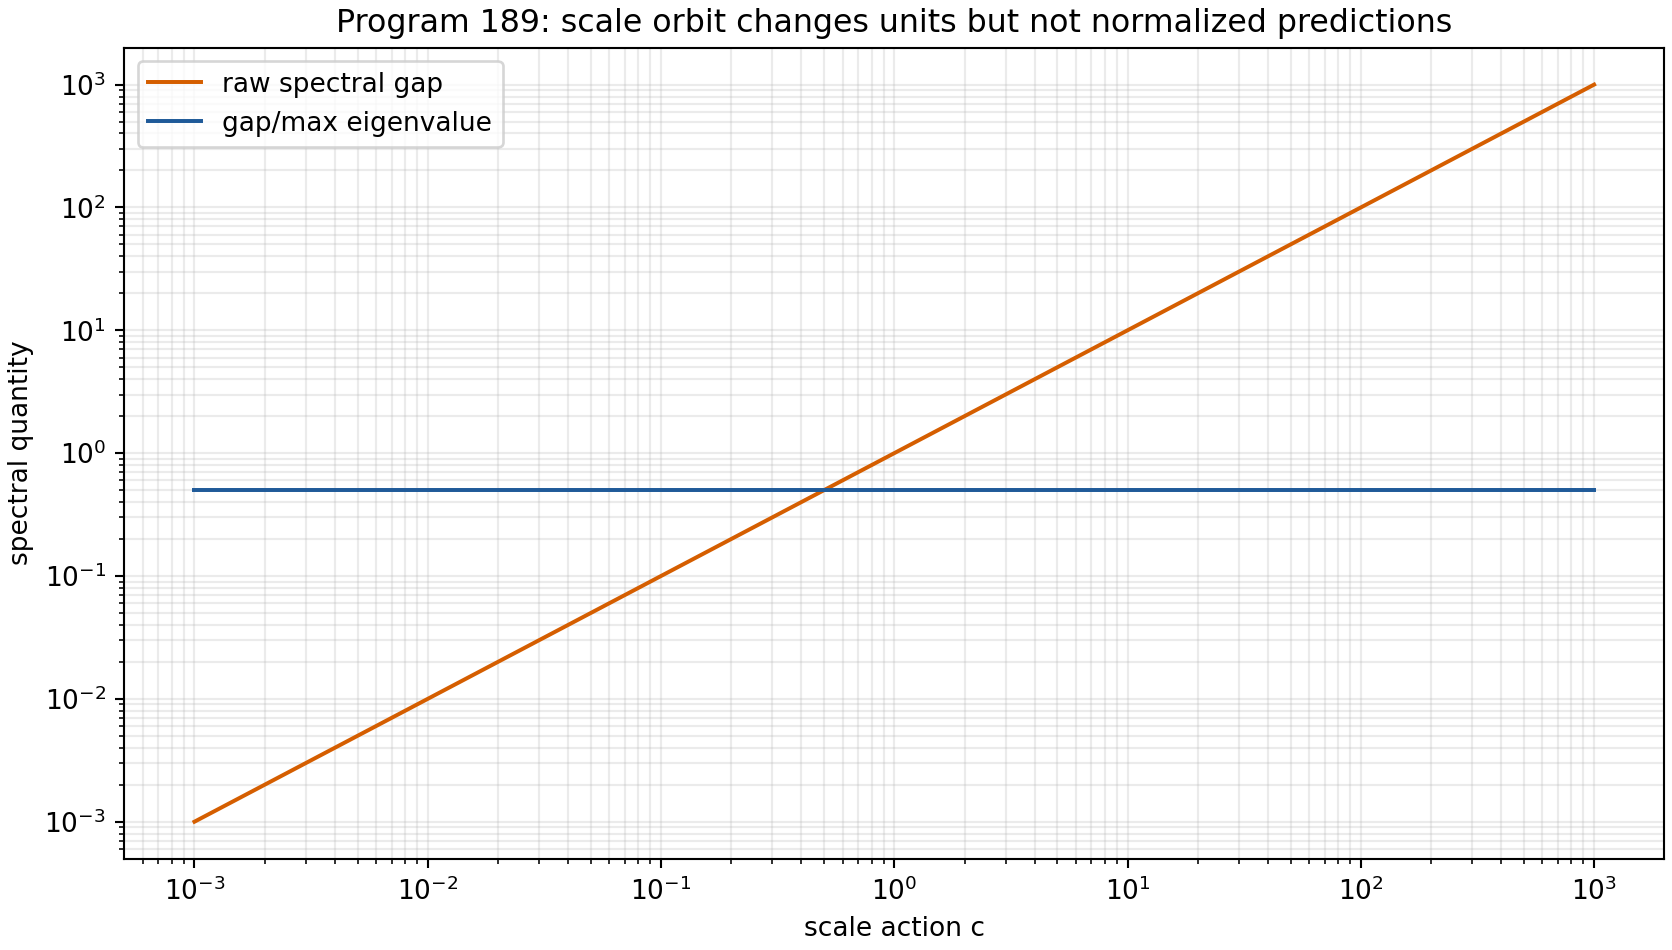
\includegraphics[width=0.94\textwidth]{FIN_Programs_178_190_Composition_Process_Scale_Figures/program189_scale_orbit.png}
\caption{Raw spectral scale changes while normalized spectral predictions remain invariant.}
\end{figure}

\section{No-section theorem}

Invariant spectral data are constant on the orbit. A rule using only such data cannot choose one representative. A scale-charged datum or calibration is necessary.

The minimal one-generator conditional object is a SpectralClockFrame, a chosen \(\tau_\ast>0\) such that

\[
\tau_\ast A
\]

is dimensionless. Under \(A\mapsto cA\) it transforms as \(\tau_\ast\mapsto\tau_\ast/c\).

\section{Verdict}

\textbf{\statusProven{}} One clock frame calibrates the spectral generator but is not a strict source. Full action, length and mass units still require a rank-three conversion package or an equivalent physical structure.

\par\medskip\hrule\medskip

\chapter{Program 190 --- External-data intake gate}

\section{Operational requirements}

The gate requires eleven fields:

\begin{enumerate}
\item 
public source identifier;

\item 
explicit license identifier;

\item 
immutable hashes;

\item 
preparation provenance;

\item 
raw time-ordered records;

\item 
physical units and timestamps;

\item 
detector calibration;

\item 
apparatus-memory calibration;

\item 
reference control;

\item 
exclusion audit;

\item 
independent analysis boundary.

\end{enumerate}

\section{Audited local bundles}

Three local candidates are checked:

\begin{itemize}
\item 
raw\_strain\_unfiltered: sixteen .h5 paths, nine valid HDF5 signatures, but no embedded units, timestamps, provenance or control metadata;

\item 
beta\_channel\_true\_external\_v2: genuine external-source statement and five present hash-listed files, but no explicit license, raw operational record, preparation or calibration compatible with this protocol;

\item 
confirmatory\_dataset\_external\_source\_rebuild: two present summary files and hashes, but generic license text and no raw operational chain.

\end{itemize}

\begin{figure}[htbp]
\centering
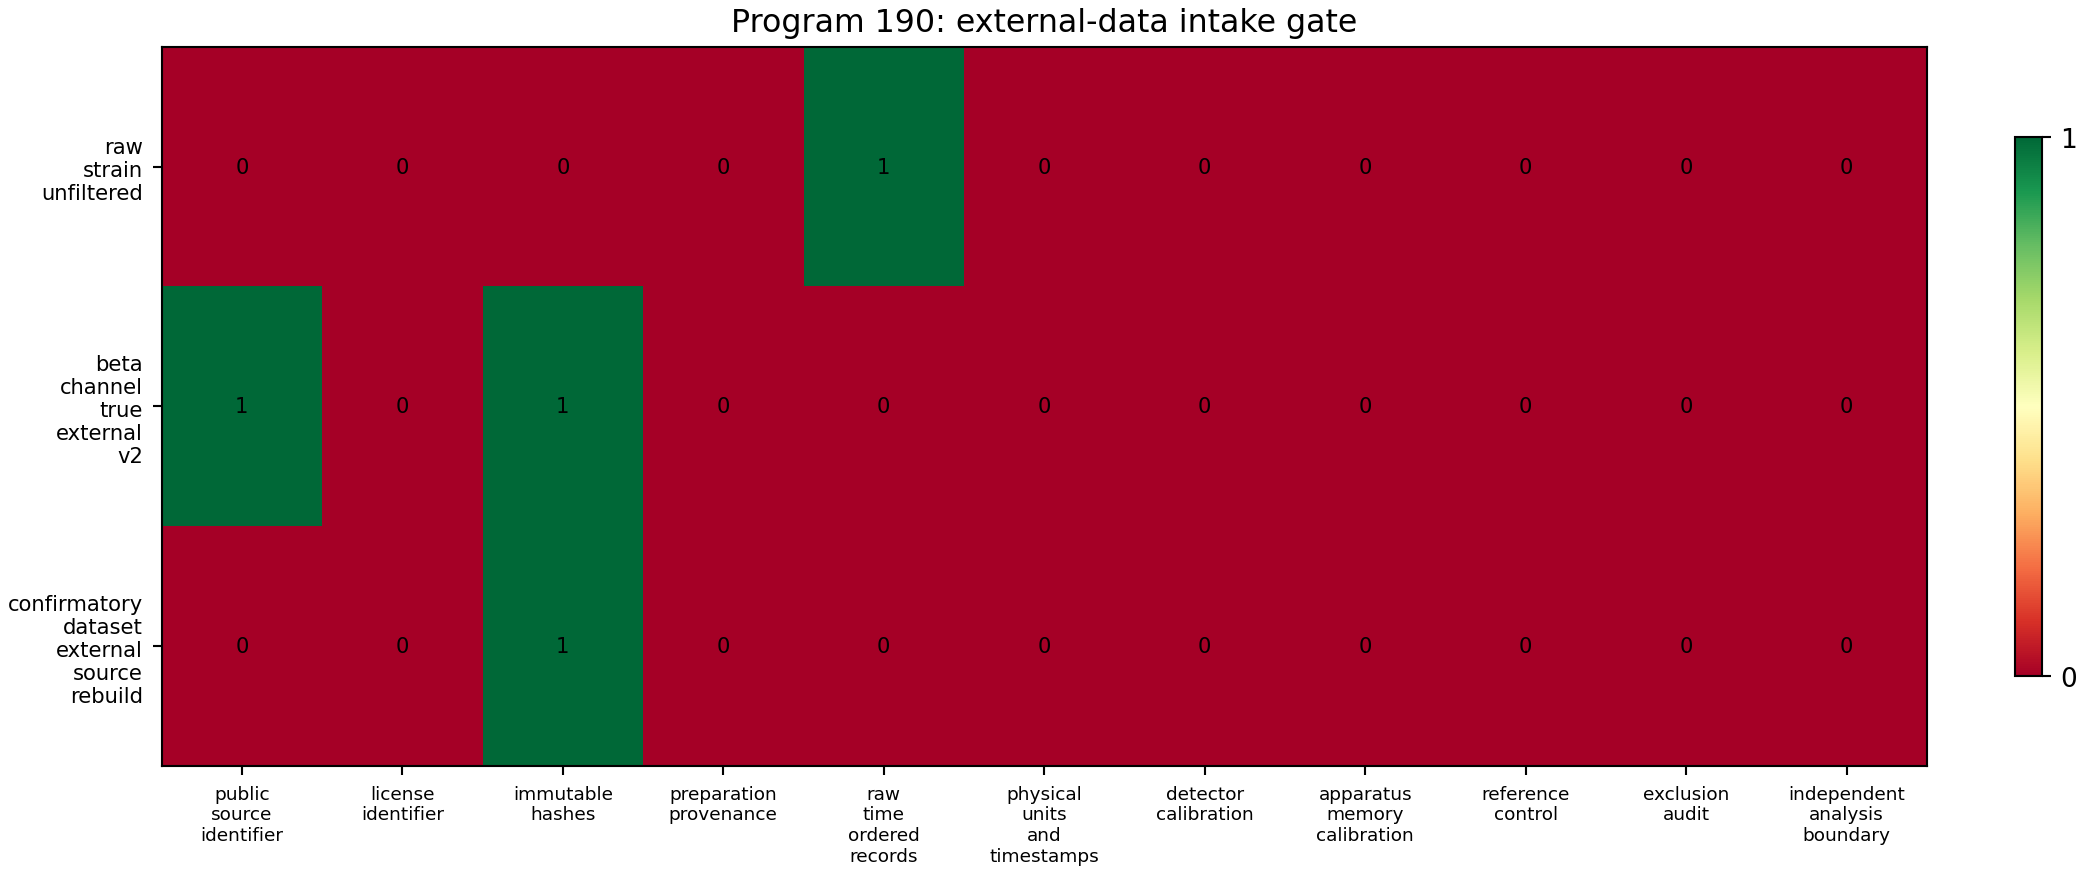
\includegraphics[width=0.94\textwidth]{FIN_Programs_178_190_Composition_Process_Scale_Figures/program190_external_intake.png}
\caption{None of three local external-lineage candidates passes the eleven-field operational intake gate.}
\end{figure}

\section{Verdict}

\textbf{[Proven local audit]} No bundle passes all eleven requirements. This does not deny that some files have authentic external provenance or value for other repository tests. It means that none is admissible for the specific state--control--detector--memory protocol constructed here.

No external result is computed, and the intake failure itself is archived as the scientific outcome.

\par\medskip\hrule\medskip

\chapter{Cross-program synthesis}

\section{Four nontrivial moduli}

The round identifies four independent families:

\[
\begin{aligned}
\mathcal M_{\rm state}
&=\{F(\alpha/\log h)\},\\
\mathcal T_{\beta}
&=\mathbb R_{>0}\text{ as a scale torsor},\\
\mathcal M_{\rm env}(A)
&=\{\text{reduced processes compatible with }A\},\\
\mathcal T_{\rm clock}
&=\{\tau_\ast>0\}.
\end{aligned}
\]

The spectral generator determines none of their representatives.

\section{What is unavoidable}

The following are unavoidable consequences of the common operator:

\begin{itemize}
\item 
spectral measure;

\item 
unitary and heat functional calculi;

\item 
resolvents;

\item 
dimensionless spectral ratios;

\item 
exact Dirichlet positivity under the graph hypotheses.

\end{itemize}

\section{What requires a section}

The following require additional data:

\begin{itemize}
\item 
a reference state or state law;

\item 
one compression/\allowbreak{}length representative;

\item 
a signed preparation;

\item 
an environment process;

\item 
memory-sensitive interventions;

\item 
a clock and dimensional conversion;

\item 
detector and record calibration.

\end{itemize}

Mathematically, the missing physical principle would have to provide compatible sections

\[
\sigma_{\rm state},\quad
\sigma_\beta,\quad
\sigma_{\rm env},\quad
\sigma_{\rm clock}
\]

and prove their naturality. Current invariant data provide no such global section.

\section{Why packaging is not derivation}

AFIS or a process tensor may package several inputs in one tuple. A completion map may reproduce the strict target. A gauge may set \(\beta=1\). None of these notations reduces the independent information required. Mathematical minimality must count the information in a specification, not the number of symbols used.

\par\medskip\hrule\medskip

\chapter{Corrected theoretical architecture}

\section{Strict informational layer}

The strict layer contains:

\[
W_0=(\mathcal H,A,E_A,\text{dimensionless kernel invariants}).
\]

It supports wave, diffusion and Green dynamics.

\section{Conditional conversion layer}

The conversion layer contains:

\[
\mathrm{CA}
=
(\tau_\ast,\ell_\ast,\hbar_\ast)
\]

or an equivalent rank-three dimensional frame. Program 189 proves that at least a clock representative is needed even for one generator.

\section{Conditional operational layer}

The operational layer contains:

\[
\mathrm{OP}
=
(\rho,\mathcal P,\Upsilon_{2:0},
\mathcal I,\mathcal D,\mathcal R),
\]

where \(\Upsilon_{2:0}\) is a process tensor, \(\mathcal I\) an intervention family, \(\mathcal D\) detector calibration and \(\mathcal R\) a record.

\section{Optional completion layer}

The kernel bridge is a separate typed object:

\[
\mathcal B:
K_{\rm legacy}+\text{new sourced data}
\longrightarrow K_{\rm strict}.
\]

Program 188 proves that the phase arrow cannot be algebraic in legacy cyclotomic data alone. Program 179 proves that the damping arrow needs a scale representative or new source.

\par\medskip\hrule\medskip

\chapter{Falsification ledger}

\section{Surviving theorems}

\begin{itemize}
\item 
common spectral functional calculus;

\item 
exact finite Dirichlet identity;

\item 
state-law moduli classification;

\item 
positive compression torsor;

\item 
complete covariant qubit conversion criterion;

\item 
exact repeated-block DKW theorem;

\item 
nonlinear calibration rank;

\item 
feature permutation-invariance no-go;

\item 
two-step memory witness;

\item 
environment nonuniqueness;

\item 
phase transcendence obstruction;

\item 
scale-orbit no-section theorem.

\end{itemize}

\section{Surviving conditional constructions}

\begin{itemize}
\item 
one-copy \(\beta_F=\log2\) state;

\item 
\(\beta=1\) coordinate gauge;

\item 
MultiControlCalibrationFrame;

\item 
TwoStepProcessInstrument;

\item 
SpectralClockFrame;

\item 
CA/\allowbreak{}operational packaging.

\end{itemize}

\section{Refuted in scope}

\begin{itemize}
\item 
unique state selection by composition and label invariance;

\item 
strict \(\beta=1\) from positivity or unitality;

\item 
completeness of scalar reflection monotone \(M\);

\item 
nominal-\(n\) DKW under repeated blocks;

\item 
general memory identification by marginal quantile features;

\item 
unique environment from \(A\);

\item 
algebraic legacy-only strict phase completion;

\item 
intrinsic scale selection by normalized spectral data.

\end{itemize}

\section{Still open}

\begin{itemize}
\item 
full Arb/\allowbreak{}acb certificate;

\item 
compiled proof-assistant generalization;

\item 
arbitrary mixing inference;

\item 
sourced scale-charged datum;

\item 
sourced sector selector;

\item 
source-complete legacy-to-strict map;

\item 
admissible external experiment.

\end{itemize}

\par\medskip\hrule\medskip

\chapter{Recommended Programs 191--203}

The following thirteen programs are ranked by expected information gain.

\section{Priority 1 --- Program 191: reference-state source theorem}

Replace scalar temperature hunting by a typed reference-state problem. Classify natural transformations assigning a faithful state to each admitted fibre algebra under tensor products and coarse graining. Determine whether normalized trace is unique and document that it yields \(17/9\), or identify the minimal extra datum needed for uniform central-sector weighting.

\section{Priority 2 --- Program 192: beta-gauge invariant bridge observables}

Work on exactly one completion atom. Introduce a conditional length frame, quotient the positive \(\beta\) torsor and classify which strict/\allowbreak{}legacy comparisons are invariant under its action. This can distinguish meaningful shape claims from coordinate-dependent \(\beta=1\) statements without claiming bridge closure.

\section{Priority 3 --- Program 193: common-engine Arb certificate}

Install or supply a reproducible Arb/\allowbreak{}python-flint environment and evaluate all five Program-180 components in one directed-rounding pipeline. The outcome must be either the formal sub-three-percent certificate or a formal lower bound on the remaining interval width.

\section{Priority 4 --- Program 194: compiled finite Dirichlet library}

Compile a proof-assistant development with general finite symmetric nonnegative \(W\), constant row sum, positivity of \(sI-W\), constant null vector, unitary exponential and positivity/\allowbreak{}stochasticity of the heat semigroup. Keep physical interpretation outside the formal theorem.

\section{Priority 5 --- Program 195: analytic reflection-conversion geometry}

Eliminate the numerical one-dimensional maximization from Program 182. Derive a closed-form boundary, classify extremal channels and study tensor composition or catalysis of the complete conversion preorder.

\section{Priority 6 --- Program 196: mixing-aware empirical process theorem}

Move beyond repeated blocks to a declared beta-mixing or martingale class. Prove a nonasymptotic quantile bound with observable acquisition assumptions, then measure the information cost relative to iid and block-valid intervals.

\section{Priority 7 --- Program 197: order-sensitive open-set protocol}

Add autocorrelation, ordinal-pattern, time-reversal and intervention-response features before retraining. Freeze an open-set risk criterion and challenge it with multiset-preserving permutations, long memory and nonstationary apparatus processes.

\section{Priority 8 --- Program 198: minimal process-tensor tomography}

Determine the smallest preparation/\allowbreak{}intervention set identifying the two-step dephasing process used in Program 186. Prove rank and conditioning, then add detector blur as a separate nuisance channel.

\section{Priority 9 --- Program 199: environment equivalence and causal}

identifiability

Classify dilation equivalence classes producing the same reduced process. Ask which environmental properties are operationally identifiable and prove that unidentifiable microscopic coordinates cannot receive physical claims.

\section{Priority 10 --- Program 200: analytic phase-source classification}

Having excluded finite algebraic legacy operations, classify analytic functional operations that could generate \(e^{i743/4000}\) without inserting the target. Require a repository-sourced argument, phase origin and coupling law. Stop if every candidate is constant or target-coded.

\section{Priority 11 --- Program 201: scale-free observable catalogue}

Construct the maximal set of predictions invariant under \((A,t,z)\mapsto(cA,t/c,cz)\). These are the only quantities testable before a physical clock is supplied. Separate scale-free falsification from dimensionful fitting.

\section{Priority 12 --- Program 202: admissible experimental bundle}

Build, acquire or document one dataset bundle containing all eleven Program-190 fields, especially preparation, raw order, detector calibration, memory calibration and a known reference control. Do not run the physics protocol until the intake hash is frozen and the license is explicit.

\section{Priority 13 --- Program 203: one conditional CA+OP prediction}

Choose one narrow observable and derive it from

\[
W_0+\mathrm{CA}+\mathrm{OP}
\]

with every imported unit and instrument parameter displayed. Compare against an admissible record only if Program 202 passes. The result must remain conditional and must not be promoted to strict FIN or ToE closure.

\section{Quantitative ranking}

\[
\begin{array}{c|c|c}
\text{rank}&\text{program}&\text{probability of decisive progress}\\
\hline
1&191&0.88\\
2&192&0.84\\
3&197&0.82\\
4&198&0.80\\
5&195&0.78\\
6&196&0.75\\
7&201&0.74\\
8&194&0.72\\
9&193&0.68\\
10&199&0.67\\
11&200&0.62\\
12&202&0.48\\
13&203&0.35
\end{array}
\]

Program 203 is ranked last only because it is logically downstream of an admissible experimental bundle. A rigorous negative result in any of the higher-ranked programs is considered decisive progress.

\par\medskip\hrule\medskip

\chapter{Final conclusion}

The attempt to make FIN physical by finding one numerically distinguished constant has now been replaced by a more precise mathematical question: which nontrivial bundles or moduli must receive sections before an experiment is defined?

The spectral generator supplies real structure. It unifies wave, diffusion and Green dynamics and supports exact Dirichlet mathematics. But composition leaves a state-law moduli space; positive compression is a scale torsor; the same generator admits a continuum of environments; process memory requires interventions; and dimensional time lives on a free positive orbit.

The new complete reflection-conversion theorem and the process-memory instrument show that progress does not require pretending these missing objects are already derived. They can be constructed, classified and tested as independent mathematical objects.

The deepest interpretation surviving this round is:

\textbf{FIN is presently a rigorous dimensionless spectral-dynamical foundation equipped with unresolved state, scale and operational section problems. Physics begins only after those sections are sourced or explicitly supplied and made falsifiable.}

That conclusion is stronger than a vague statement that "more physics is needed." It identifies the precise mathematical types of the missing data and proves that several natural invariant constructions cannot provide them.

\par\medskip\hrule\medskip

\chapter{Reproducibility statement}

The executable, 72 tests, machine-readable results, preregistration, finite Lean source and thirteen figures are included. All stochastic studies use a fixed seed. Firecrawl and external web access were not used. Repository-local external-lineage files were inspected only by the Program-190 intake gate; no external physical validation was executed.

\chapter{Suggested citation}

\.Zuchowski, K. (2026). \emph{FIN Programs 178--190: Composition Laws, Process Memory, and Scale Obstructions} (FIN Research Monograph, Release 10.17; Version 1.0.0) [Preprint]. Zenodo.


\clearpage
\chapter*{Archival note}
\addcontentsline{toc}{chapter}{Archival note}
Machine-readable results are stored in
\path{FIN_Programs_178_190_Composition_Process_Scale_Results.json}.
The frozen open-set challenge is stored in
\path{FIN_Programs_178_190_Open_Set_Preregistration.json}.
The executable, seventy-two tests, finite Lean source, and thirteen figures
reproduce the declared release scope.

\medskip
\noindent\textbf{Suggested citation:}

\.Zuchowski, K. (2026). \emph{FIN Programs 178--190: Composition Laws,
Process Memory, and Scale Obstructions}
(FIN Research Monograph, Release 10.17; Version 1.0.0) [Preprint]. Zenodo.
\end{document}
